%% bare_jrnl.tex
%% V1.4b
%% 2015/08/26
%% by Michael Shell
%% see http://www.michaelshell.org/
%% for current contact information.
%%
%% This is a skeleton file demonstrating the use of IEEEtran.cls
%% (requires IEEEtran.cls version 1.8b or later) with an IEEE
%% journal paper.
%%
%% Support sites:
%% http://www.michaelshell.org/tex/ieeetran/
%% http://www.ctan.org/pkg/ieeetran
%% and
%% http://www.ieee.org/

%%*************************************************************************
%% Legal Notice:
%% This code is offered as-is without any warranty either expressed or
%% implied; without even the implied warranty of MERCHANTABILITY or
%% FITNESS FOR A PARTICULAR PURPOSE! 
%% User assumes all risk.
%% In no event shall the IEEE or any contributor to this code be liable for
%% any damages or losses, including, but not limited to, incidental,
%% consequential, or any other damages, resulting from the use or misuse
%% of any information contained here.
%%
%% All comments are the opinions of their respective authors and are not
%% necessarily endorsed by the IEEE.
%%
%% This work is distributed under the LaTeX Project Public License (LPPL)
%% ( http://www.latex-project.org/ ) version 1.3, and may be freely used,
%% distributed and modified. A copy of the LPPL, version 1.3, is included
%% in the base LaTeX documentation of all distributions of LaTeX released
%% 2003/12/01 or later.
%% Retain all contribution notices and credits.
%% ** Modified files should be clearly indicated as such, including  **
%% ** renaming them and changing author support contact information. **
%%*************************************************************************


% *** Authors should verify (and, if needed, correct) their LaTeX system  ***
% *** with the testflow diagnostic prior to trusting their LaTeX platform ***
% *** with production work. The IEEE's font choices and paper sizes can   ***
% *** trigger bugs that do not appear when using other class files.       ***                          ***
% The testflow support page is at:
% http://www.michaelshell.org/tex/testflow/



\documentclass[journal]{IEEEtran}
%
% If IEEEtran.cls has not been installed into the LaTeX system files,
% manually specify the path to it like:
% \documentclass[journal]{../sty/IEEEtran}

% --- Encoding & basic packages added for this paper ---
\usepackage[T1]{fontenc}
\usepackage[utf8]{inputenc}
\usepackage{amsmath}
\usepackage{amssymb}
\usepackage{textcomp}
\usepackage{url}
\usepackage{graphicx}
\graphicspath{{../out/plots/}}
\usepackage[colorlinks=true,urlcolor=blue,linkcolor=black,citecolor=black]{hyperref}





% Some very useful LaTeX packages include:
% (uncomment the ones you want to load)


% *** MISC UTILITY PACKAGES ***
%
%\usepackage{ifpdf}
% Heiko Oberdiek's ifpdf.sty is very useful if you need conditional
% compilation based on whether the output is pdf or dvi.
% usage:
% \ifpdf
%   % pdf code
% \else
%   % dvi code
% \fi
% The latest version of ifpdf.sty can be obtained from:
% http://www.ctan.org/pkg/ifpdf
% Also, note that IEEEtran.cls V1.7 and later provides a builtin
% \ifCLASSINFOpdf conditional that works the same way.
% When switching from latex to pdflatex and vice-versa, the compiler may
% have to be run twice to clear warning/error messages.






% *** CITATION PACKAGES ***
%
%\usepackage{cite}
% cite.sty was written by Donald Arseneau
% V1.6 and later of IEEEtran pre-defines the format of the cite.sty package
% \cite{} output to follow that of the IEEE. Loading the cite package will
% result in citation numbers being automatically sorted and properly
% "compressed/ranged". e.g., [1], [9], [2], [7], [5], [6] without using
% cite.sty will become [1], [2], [5]--[7], [9] using cite.sty. cite.sty's
% \cite will automatically add leading space, if needed. Use cite.sty's
% noadjust option (cite.sty V3.8 and later) if you want to turn this off
% such as if a citation ever needs to be enclosed in parenthesis.
% cite.sty is already installed on most LaTeX systems. Be sure and use
% version 5.0 (2009-03-20) and later if using hyperref.sty.
% The latest version can be obtained at:
% http://www.ctan.org/pkg/cite
% The documentation is contained in the cite.sty file itself.






% *** GRAPHICS RELATED PACKAGES ***
%
\ifCLASSINFOpdf
  % \usepackage[pdftex]{graphicx}
  % declare the path(s) where your graphic files are
  % \graphicspath{{../pdf/}{../jpeg/}}
  % and their extensions so you won't have to specify these with
  % every instance of \includegraphics
  % \DeclareGraphicsExtensions{.pdf,.jpeg,.png}
\else
  % or other class option (dvipsone, dvipdf, if not using dvips). graphicx
  % will default to the driver specified in the system graphics.cfg if no
  % driver is specified.
  % \usepackage[dvips]{graphicx}
  % declare the path(s) where your graphic files are
  % \graphicspath{{../eps/}}
  % and their extensions so you won't have to specify these with
  % every instance of \includegraphics
  % \DeclareGraphicsExtensions{.eps}
\fi
% graphicx was written by David Carlisle and Sebastian Rahtz. It is
% required if you want graphics, photos, etc. graphicx.sty is already
% installed on most LaTeX systems. The latest version and documentation
% can be obtained at: 
% http://www.ctan.org/pkg/graphicx
% Another good source of documentation is "Using Imported Graphics in
% LaTeX2e" by Keith Reckdahl which can be found at:
% http://www.ctan.org/pkg/epslatex
%
% latex, and pdflatex in dvi mode, support graphics in encapsulated
% postscript (.eps) format. pdflatex in pdf mode supports graphics
% in .pdf, .jpeg, .png and .mps (metapost) formats. Users should ensure
% that all non-photo figures use a vector format (.eps, .pdf, .mps) and
% not a bitmapped formats (.jpeg, .png). The IEEE frowns on bitmapped formats
% which can result in "jaggedy"/blurry rendering of lines and letters as
% well as large increases in file sizes.
%
% You can find documentation about the pdfTeX application at:
% http://www.tug.org/applications/pdftex





% *** MATH PACKAGES ***
%
%\usepackage{amsmath}
% A popular package from the American Mathematical Society that provides
% many useful and powerful commands for dealing with mathematics.
%
% Note that the amsmath package sets \interdisplaylinepenalty to 10000
% thus preventing page breaks from occurring within multiline equations. Use:
%\interdisplaylinepenalty=2500
% after loading amsmath to restore such page breaks as IEEEtran.cls normally
% does. amsmath.sty is already installed on most LaTeX systems. The latest
% version and documentation can be obtained at:
% http://www.ctan.org/pkg/amsmath





% *** SPECIALIZED LIST PACKAGES ***
%
%\usepackage{algorithmic}
% algorithmic.sty was written by Peter Williams and Rogerio Brito.
% This package provides an algorithmic environment fo describing algorithms.
% You can use the algorithmic environment in-text or within a figure
% environment to provide for a floating algorithm. Do NOT use the algorithm
% floating environment provided by algorithm.sty (by the same authors) or
% algorithm2e.sty (by Christophe Fiorio) as the IEEE does not use dedicated
% algorithm float types and packages that provide these will not provide
% correct IEEE style captions. The latest version and documentation of
% algorithmic.sty can be obtained at:
% http://www.ctan.org/pkg/algorithms
% Also of interest may be the (relatively newer and more customizable)
% algorithmicx.sty package by Szasz Janos:
% http://www.ctan.org/pkg/algorithmicx




% *** ALIGNMENT PACKAGES ***
%
%\usepackage{array}
% Frank Mittelbach's and David Carlisle's array.sty patches and improves
% the standard LaTeX2e array and tabular environments to provide better
% appearance and additional user controls. As the default LaTeX2e table
% generation code is lacking to the point of almost being broken with
% respect to the quality of the end results, all users are strongly
% advised to use an enhanced (at the very least that provided by array.sty)
% set of table tools. array.sty is already installed on most systems. The
% latest version and documentation can be obtained at:
% http://www.ctan.org/pkg/array


% IEEEtran contains the IEEEeqnarray family of commands that can be used to
% generate multiline equations as well as matrices, tables, etc., of high
% quality.




% *** SUBFIGURE PACKAGES ***
%\ifCLASSOPTIONcompsoc
%  \usepackage[caption=false,font=normalsize,labelfont=sf,textfont=sf]{subfig}
%\else
%  \usepackage[caption=false,font=footnotesize]{subfig}
%\fi
% subfig.sty, written by Steven Douglas Cochran, is the modern replacement
% for subfigure.sty, the latter of which is no longer maintained and is
% incompatible with some LaTeX packages including fixltx2e. However,
% subfig.sty requires and automatically loads Axel Sommerfeldt's caption.sty
% which will override IEEEtran.cls' handling of captions and this will result
% in non-IEEE style figure/table captions. To prevent this problem, be sure
% and invoke subfig.sty's "caption=false" package option (available since
% subfig.sty version 1.3, 2005/06/28) as this is will preserve IEEEtran.cls
% handling of captions.
% Note that the Computer Society format requires a larger sans serif font
% than the serif footnote size font used in traditional IEEE formatting
% and thus the need to invoke different subfig.sty package options depending
% on whether compsoc mode has been enabled.
%
% The latest version and documentation of subfig.sty can be obtained at:
% http://www.ctan.org/pkg/subfig




% *** FLOAT PACKAGES ***
%
%\usepackage{fixltx2e}
% fixltx2e, the successor to the earlier fix2col.sty, was written by
% Frank Mittelbach and David Carlisle. This package corrects a few problems
% in the LaTeX2e kernel, the most notable of which is that in current
% LaTeX2e releases, the ordering of single and double column floats is not
% guaranteed to be preserved. Thus, an unpatched LaTeX2e can allow a
% single column figure to be placed prior to an earlier double column
% figure.
% Be aware that LaTeX2e kernels dated 2015 and later have fixltx2e.sty's
% corrections already built into the system in which case a warning will
% be issued if an attempt is made to load fixltx2e.sty as it is no longer
% needed.
% The latest version and documentation can be found at:
% http://www.ctan.org/pkg/fixltx2e


%\usepackage{stfloats}
% stfloats.sty was written by Sigitas Tolusis. This package gives LaTeX2e
% the ability to do double column floats at the bottom of the page as well
% as the top. (e.g., "\begin{figure*}[!b]" is not normally possible in
% LaTeX2e). It also provides a command:
%\fnbelowfloat
% to enable the placement of footnotes below bottom floats (the standard
% LaTeX2e kernel puts them above bottom floats). This is an invasive package
% which rewrites many portions of the LaTeX2e float routines. It may not work
% with other packages that modify the LaTeX2e float routines. The latest
% version and documentation can be obtained at:
% http://www.ctan.org/pkg/stfloats
% Do not use the stfloats baselinefloat ability as the IEEE does not allow
% \baselineskip to stretch. Authors submitting work to the IEEE should note
% that the IEEE rarely uses double column equations and that authors should try
% to avoid such use. Do not be tempted to use the cuted.sty or midfloat.sty
% packages (also by Sigitas Tolusis) as the IEEE does not format its papers in
% such ways.
% Do not attempt to use stfloats with fixltx2e as they are incompatible.
% Instead, use Morten Hogholm'a dblfloatfix which combines the features
% of both fixltx2e and stfloats:
%
% \usepackage{dblfloatfix}
% The latest version can be found at:
% http://www.ctan.org/pkg/dblfloatfix




%\ifCLASSOPTIONcaptionsoff
%  \usepackage[nomarkers]{endfloat}
% \let\MYoriglatexcaption\caption
% \renewcommand{\caption}[2][\relax]{\MYoriglatexcaption[#2]{#2}}
%\fi
% endfloat.sty was written by James Darrell McCauley, Jeff Goldberg and 
% Axel Sommerfeldt. This package may be useful when used in conjunction with 
% IEEEtran.cls'  captionsoff option. Some IEEE journals/societies require that
% submissions have lists of figures/tables at the end of the paper and that
% figures/tables without any captions are placed on a page by themselves at
% the end of the document. If needed, the draftcls IEEEtran class option or
% \CLASSINPUTbaselinestretch interface can be used to increase the line
% spacing as well. Be sure and use the nomarkers option of endfloat to
% prevent endfloat from "marking" where the figures would have been placed
% in the text. The two hack lines of code above are a slight modification of
% that suggested by in the endfloat docs (section 8.4.1) to ensure that
% the full captions always appear in the list of figures/tables - even if
% the user used the short optional argument of \caption[]{}.
% IEEE papers do not typically make use of \caption[]'s optional argument,
% so this should not be an issue. A similar trick can be used to disable
% captions of packages such as subfig.sty that lack options to turn off
% the subcaptions:
% For subfig.sty:
% \let\MYorigsubfloat\subfloat
% \renewcommand{\subfloat}[2][\relax]{\MYorigsubfloat[]{#2}}
% However, the above trick will not work if both optional arguments of
% the \subfloat command are used. Furthermore, there needs to be a
% description of each subfigure *somewhere* and endfloat does not add
% subfigure captions to its list of figures. Thus, the best approach is to
% avoid the use of subfigure captions (many IEEE journals avoid them anyway)
% and instead reference/explain all the subfigures within the main caption.
% The latest version of endfloat.sty and its documentation can obtained at:
% http://www.ctan.org/pkg/endfloat
%
% The IEEEtran \ifCLASSOPTIONcaptionsoff conditional can also be used
% later in the document, say, to conditionally put the References on a 
% page by themselves.




% *** PDF, URL AND HYPERLINK PACKAGES ***
%
%\usepackage{url}
% url.sty was written by Donald Arseneau. It provides better support for
% handling and breaking URLs. url.sty is already installed on most LaTeX
% systems. The latest version and documentation can be obtained at:
% http://www.ctan.org/pkg/url
% Basically, \url{my_url_here}.




% *** Do not adjust lengths that control margins, column widths, etc. ***
% *** Do not use packages that alter fonts (such as pslatex).         ***
% There should be no need to do such things with IEEEtran.cls V1.6 and later.
% (Unless specifically asked to do so by the journal or conference you plan
% to submit to, of course. )


% correct bad hyphenation here
\hyphenation{op-tical net-works semi-conduc-tor}


\begin{document}
%
% paper title
% Titles are generally capitalized except for words such as a, an, and, as,
% at, but, by, for, in, nor, of, on, or, the, to and up, which are usually
% not capitalized unless they are the first or last word of the title.
% Linebreaks \\ can be used within to get better formatting as desired.
% Do not put math or special symbols in the title.
\title{Detecting Clinical and Social Impacts of Substance Use in Social Media:\\
A Comparative Study of Encoder-, LLM-, and SVM-Based NER Pipelines}
%
%
% author names and IEEE memberships
% note positions of commas and nonbreaking spaces ( ~ ) LaTeX will not break
% a structure at a ~ so this keeps an author's name from being broken across
% two lines.
% use \thanks{} to gain access to the first footnote area
% a separate \thanks must be used for each paragraph as LaTeX2e's \thanks
% was not built to handle multiple paragraphs
%

\author{Vlad-Ioan~B\^irsan%
\thanks{The full source code, configuration files, and trained-model
checkpoints used to produce the experiments reported in this paper are
publicly available at \protect\url{https://github.com/vl4dio4n/SMM4H-HeaRD-2026-Task-7}.}}

% note the % following the last \IEEEmembership and also \thanks - 
% these prevent an unwanted space from occurring between the last author name
% and the end of the author line. i.e., if you had this:
% 
% \author{....lastname \thanks{...} \thanks{...} }
%                     ^------------^------------^----Do not want these spaces!
%
% a space would be appended to the last name and could cause every name on that
% line to be shifted left slightly. This is one of those "LaTeX things". For
% instance, "\textbf{A} \textbf{B}" will typeset as "A B" not "AB". To get
% "AB" then you have to do: "\textbf{A}\textbf{B}"
% \thanks is no different in this regard, so shield the last } of each \thanks
% that ends a line with a % and do not let a space in before the next \thanks.
% Spaces after \IEEEmembership other than the last one are OK (and needed) as
% you are supposed to have spaces between the names. For what it is worth,
% this is a minor point as most people would not even notice if the said evil
% space somehow managed to creep in.



% The paper headers
\markboth{LLMs for NLP Course Project,~University of Bucharest,~2026}%
{B\^irsan: NER of Clinical and Social Impacts of Substance Use in Social Media}
% The only time the second header will appear is for the odd numbered pages
% after the title page when using the twoside option.
% 
% *** Note that you probably will NOT want to include the author's ***
% *** name in the headers of peer review papers.                   ***
% You can use \ifCLASSOPTIONpeerreview for conditional compilation here if
% you desire.




% If you want to put a publisher's ID mark on the page you can do it like
% this:
%\IEEEpubid{0000--0000/00\$00.00~\copyright~2015 IEEE}
% Remember, if you use this you must call \IEEEpubidadjcol in the second
% column for its text to clear the IEEEpubid mark.



% use for special paper notices
%\IEEEspecialpapernotice{(Invited Paper)}




% make the title area
\maketitle

% As a general rule, do not put math, special symbols or citations
% in the abstract or keywords.
\begin{abstract}
Nonmedical opioid use is a persistent public-health issue across most
developed countries, and the anonymity afforded by social media leads many
affected individuals to share first-person testimonies that mention both
\emph{clinical impacts} (e.g., withdrawal, addiction, the need for medical
assistance) and \emph{social impacts} (e.g., legal trouble, family conflict,
job loss, financial hardship). Automatically detecting these mentions in
user-generated text is a meaningful first step toward early intervention and
reintegration support. In this work, we investigate token-level Named Entity
Recognition for clinical and social impacts of substance use in Reddit posts,
in the context of the SMM4H-HeaRD~2026 Task~7 shared task, and compare four
families of approaches: (i) a \textbf{direct} pipeline, in which a single
encoder produces 5-class BIO tags, evaluated across several pretrained
backbones, loss functions, and an optional CRF decoding head;
(ii) a \textbf{two-stage} pipeline, in which a 3-class encoder detects
impact spans and a Large Language Model subsequently classifies each span
as Clinical, Social, or Neither, in both zero-shot and few-shot regimes;
(iii) an \textbf{audit} pipeline, in which an LLM verifies or corrects,
span by span, the predictions of a 5-class encoder (again zero- and
few-shot); and (iv) a \textbf{lightweight classical-ML variant}, in which
the LLM in pipelines (ii) and (iii) is replaced by an SVM head trained on
encoder span embeddings. Our best configuration, a DeBERTa-v3 encoder with
a CRF decoding head, attains $45.38\%$ strict micro-F1 and $54.20\%$ relaxed
overlap F1 on the official Codabench test set. None of our configurations
surpasses the shared-task baseline reported by Dey~\emph{et~al.}~\cite{dey2025inference},
but the cross-pipeline ablation yields concrete evidence on where encoder-only
models, LLM-based type classification, LLM-based auditing, and lightweight
SVM classifiers each help or hurt.
\end{abstract}

% Note that keywords are not normally used for peerreview papers.
\begin{IEEEkeywords}
Named Entity Recognition, substance use, opioid epidemic, social media,
BIO tagging, Conditional Random Fields, Large Language Models, few-shot
prompting, SMM4H-HeaRD.
\end{IEEEkeywords}






% For peer review papers, you can put extra information on the cover
% page as needed:
% \ifCLASSOPTIONpeerreview
% \begin{center} \bfseries EDICS Category: 3-BBND \end{center}
% \fi
%
% For peerreview papers, this IEEEtran command inserts a page break and
% creates the second title. It will be ignored for other modes.
\IEEEpeerreviewmaketitle



\section{Introduction}
\label{sec:introduction}
\IEEEPARstart{N}{onmedical} use of prescription and street opioids is a
public-health problem in most developed countries, with a high burden
among young and working-age adults. Epidemiological studies have
characterised the affected demographics and their social drivers, but
tools for the early identification, prevention, and remediation of
opioid-related harms remain limited. Over the last years a new
source of data has emerged: the personal accounts that users post on
social media. The anonymity offered by platforms such as Reddit lowers
the barrier to self-disclosure, so affected individuals describe their
substance-use experiences in detail and without fear of stigma. Social
media therefore forms a rich corpus for training systems that flag
users who have already suffered substance-use consequences --- a first
step toward timely intervention.

This work presents a comparative study of methods for extracting
clinical and social impacts of nonmedical opioid use from first-person
social-media posts. The study is conducted in the context of the
SMM4H-HeaRD~2026 Task~7 shared task, which provides a corpus of
Reddit posts annotated under a BIO tagging scheme with two entity
types: \emph{ClinicalImpacts} --- physical or psychological
consequences such as overdose, withdrawal, depression, or anxiety ---
and \emph{SocialImpacts} --- relational, occupational, or legal
consequences such as job loss, legal charges, or financial hardship.
Only \emph{first-person, self-reported} impacts are annotated, which
makes the task harder than generic biomedical NER: a system has to
separate confessional posts (\emph{``I withdrew really bad''}) from
third-person reports (\emph{``my friend overdosed''}), which must
remain untagged. Performance is reported with two metrics:
\emph{strict micro-F1}, which requires exact agreement on both
boundaries and label, and \emph{relaxed overlap F1}, which credits any
non-empty overlap with a gold span of the same type.

Within this setup, we organise our study around two research
questions:

\noindent\textbf{RQ1.} Does decoupling \emph{span detection} from
\emph{span typing}, by first locating impact spans with a 3-class
encoder and then assigning their type with a downstream classifier,
improve span-level F1 over a single 5-class encoder trained
end-to-end?

\noindent\textbf{RQ2.} When span detection is already performed by a
strong 5-class encoder, can a Large Language Model audit and correct
its predictions, and is the gain (if any) larger than what a Support
Vector Machine head can achieve on the same encoder span embeddings?

To answer these questions we evaluate four families of pipelines:
(i)~a \textbf{direct} pipeline, in which a fine-tuned encoder produces
5-class BIO predictions, with an optional Conditional Random Field
decoding head; (ii)~a \textbf{two-stage} pipeline, in which a 3-class
encoder detects impact spans and an LLM labels each span as Clinical,
Social, or Neither; (iii)~an \textbf{audit} pipeline, in which an LLM
verifies and, when needed, corrects the predictions of a 5-class
encoder, span by span; and (iv)~an \textbf{SVM-based variant}, in
which the LLM in (ii) and (iii) is replaced by a Support Vector
Machine head trained on encoder span embeddings. Each family is run
across several encoder backbones, training losses, and both zero-shot
and few-shot LLM regimes. None of our configurations surpasses the
DeBERTa-large baseline reported by the shared-task
organisers~\cite{dey2025inference}, but the cross-pipeline ablation
addresses both research questions and shows where each design choice
helps or hurts.

The remainder of the paper is organised as follows.
Section~\ref{sec:related} reviews related work and the building blocks
of our pipelines. Section~\ref{sec:methodology} describes the dataset
and the design of each system. Section~\ref{sec:experiments} reports
the experimental setup, Section~\ref{sec:results} the results and a
comparison across methods, and Section~\ref{sec:conclusion} concludes
with limitations and directions for future work.

\section{Related Work}
\label{sec:related}
The work in this paper sits at the intersection of three strands of
research: (i) domain-specific NER for substance-use text, (ii)
pretrained transformer encoders fine-tuned for token classification,
and (iii) instruction-tuned Large Language Models used as in-context
classifiers. We review them in this order before describing how the
field falls short.

\subsection{Substance-use NER and the SMM4H-HeaRD task}
Public-health monitoring on social media has been studied for many
years, but most work targets symptom or drug-name extraction rather
than self-reported consequences. The dataset and the baseline used in
this paper come from Dey~\emph{et~al.}~\cite{dey2025inference}, who
introduced the SMM4H-HeaRD~2026 Task~7 corpus of Reddit posts
annotated with first-person clinical and social impacts of nonmedical
opioid use, and who report a fine-tuned DeBERTa-large baseline at
$0.61$ relaxed F1. The same authors document a gap between expert
annotators and current models: clinical professionals reach high
agreement, while encoder-only systems struggle with implicit and
figurative descriptions of impacts (e.g.~``I lost everything''). Their
dataset is small (around $1{,}700$ annotated segments), imbalanced
toward the \texttt{O} class, and biased toward English-speaking
subreddits, which limits generalisation. Following Tjong Kim Sang and
De~Meulder~\cite{tjong2003conll}, both the dataset and our evaluation
adopt BIO tagging and span-level F1; we additionally distinguish
\emph{strict} F1 (exact span and label match) from \emph{relaxed} F1
(any non-empty overlap with a gold span of the same type), the
convention used by the shared task and implemented by
\texttt{seqeval}.

\subsection{Pretrained transformer encoders}
All four of our pipelines build on the encoder fine-tuning recipe
introduced with BERT~\cite{devlin2019bert} and refined by
RoBERTa~\cite{liu2019roberta}, which removes the next-sentence
prediction objective and trains for longer on more data. Our baseline
encoder (Exp~01--02b) is \texttt{mental-roberta-base}, the RoBERTa
checkpoint domain-adapted to mental-health Reddit text by
Ji~\emph{et~al.} alongside MentalBERT~\cite{ji2022mentalbert}; the
same authors show that mental-health domain adaptation helps on
Reddit-style text, which motivates this choice for an opioid-related
corpus. Our second encoder is DeBERTa-v3~\cite{he2023debertav3},
which combines disentangled attention with ELECTRA-style
replaced-token-detection pre-training and outperforms RoBERTa on GLUE
and SuperGLUE; this is the backbone for Experiments~03--05 and
09--10.

\subsection{Sequence labelling and CRF decoding}
Conditional Random Fields~\cite{lafferty2001crf} are the standard
probabilistic model for joint sequence labelling: they assign a
globally normalised score to a full label sequence and admit exact
decoding via the Viterbi algorithm.
Lample~\emph{et~al.}~\cite{lample2016neural} introduced the canonical
recipe of pairing a neural encoder with a linear-chain CRF head to
enforce valid BIO transitions (e.g.~\texttt{I-Clinical} cannot follow
\texttt{B-Social} or \texttt{O}). Our Exp~04 follows the same pattern,
replacing the original BiLSTM with DeBERTa-v3, and serves as the
strongest encoder-only system in our ablation.

\subsection{Training techniques on small, imbalanced data}
Token-level NER on small and imbalanced datasets benefits from two
training techniques that are now common in the literature. Focal
loss~\cite{lin2017focal}, originally proposed for dense object
detection, down-weights easy negatives and concentrates the gradient
on hard, rare classes; we apply it in Experiments~02b, 03, and 05a,
where the \texttt{O} tag dominates by a factor of about $16{:}1$ on
the training split.
Discriminative or layer-wise learning-rate decay (LLRD), introduced
for transfer learning by Howard and Ruder~\cite{howard2018ulmfit},
applies smaller learning rates to lower transformer layers and larger
rates to the task-specific head. LLRD is widely reported to stabilise
DeBERTa fine-tuning and we use it in every DeBERTa-based experiment.

\subsection{LLMs as in-context span classifiers}
Brown~\emph{et~al.}~\cite{brown2020fewshot} popularised the in-context
learning paradigm in which a frozen autoregressive language model is
conditioned on a task description and a small number of input--output
demonstrations and produces predictions without any parameter update.
Our two-stage and audit pipelines (Experiments~05a, 05b, 07--09)
instantiate this recipe on \texttt{Qwen2.5-7B-Instruct} and
\texttt{Gemma-3-12B-it}, run in 4-bit NF4 precision via the
\texttt{bitsandbytes} integration of QLoRA~\cite{dettmers2023qlora} so
that each model fits on a single 16~GB consumer GPU. The few-shot
variants supply $k{=}4$ gold span--label pairs per class, mined from
the training split, while the zero-shot variants rely solely on the
task description. As a controlled, classical-ML alternative to the
LLM, we also experiment (Exp~10) with a Support Vector
Machine~\cite{cortes1995svm} trained on encoder span embeddings; this
makes it possible to test how much of the LLM's contribution comes
from world knowledge that is not already linearly accessible in the
encoder's representation.

\subsection{Where the field falls short}
Three shortcomings recur across these works. First, the available
datasets are small and English-biased; Dey~\emph{et~al.} explicitly
note that scaling annotation requires medical expertise and is
therefore expensive~\cite{dey2025inference}, which is a fundamental
bottleneck for any supervised approach. Second, evaluation metrics
privilege exact spans, penalising systems for borderline disagreements
that human experts also disagree on; relaxed F1 mitigates but does not
remove this issue. Third, current encoder models exhibit weak
compositional understanding of implicit references, idioms, and
subreddit-specific slang --- a gap that LLMs partly close at large
inference cost. The four pipelines compared in this paper are designed
to probe whether that cost is justified, and to map the trade-off
between encoder-only structured prediction, LLM-based reasoning, and
classical-ML span classifiers.

\section{Methodology}
\label{sec:methodology}
This section first describes the SMM4H-HeaRD~2026 Task~7 corpus and
the dataset properties that drove our design choices, and then
outlines the four pipelines we built on top of it. Detailed
configurations and hyper-parameters are reported in
Section~\ref{sec:experiments}.

\subsection{Dataset}
\label{ssec:dataset}
\subsubsection{Source and purpose}
The dataset is the SMM4H-HeaRD~2026 Task~7 corpus released by
Dey~\emph{et~al.}~\cite{dey2025inference}. It was collected from
opioid-related Reddit communities and annotated by clinical experts to
support the extraction of self-reported clinical and social impacts of
nonmedical opioid use. The organisers report a total of $1{,}378$
posts and $1{,}778$ entity tokens; per-split counts are summarised in
Table~\ref{tab:dataset_stats}. The released CSVs that we use during
training and inference contain $842$ training, $258$ development, and
$578$ test rows. Train and dev are essentially one row per post (a
handful of training posts are split into multiple sentence-level
rows, so $842$ rows correspond to $743$ unique post IDs), while the
test split breaks each original post into roughly two segments so
that long posts fit into the encoder's context window. Each row
contains (i)~a list of \texttt{tokens}, (ii)~a \texttt{ner\_tags}
sequence of equal length under the BIO scheme defined in
Section~\ref{sec:related}, and (iii)~an \texttt{ID}; the post title
and source subreddit are inlined as the first few tokens of every
row. The test split is unannotated and used for blind submission to
the official Codabench leaderboard.

\begin{table}[!t]
\renewcommand{\arraystretch}{1.2}
\caption{Per-split statistics of the SMM4H-HeaRD~2026 Task~7 corpus,
as reported by the shared-task organisers. Entity columns count
\emph{tokens}, not spans.}
\label{tab:dataset_stats}
\centering
\begin{tabular}{l r r r r r}
\hline
\textbf{Split} & \textbf{Posts} & \textbf{Social} & \textbf{Clinical}
               & \textbf{All entity} & \textbf{Tokens} \\
\hline
Train  & 842   & 408 & 616 & 1{,}024 & 17.2K \\
Dev    & 258   & 167 & 223 & 390     & 5.2K \\
Test   & 278   & 256 & 108 & 364     & 6.2K \\
\hline
Total  & 1{,}378 & 831 & 947 & 1{,}778 & 28.6K \\
\hline
\end{tabular}
\end{table}

\subsubsection{Class imbalance}
Token-level statistics (Fig.~\ref{fig:class_dist}) show that the
\texttt{O} tag covers $\sim$$16{,}200$ training tokens against only
$\sim$$1{,}024$ tokens for the four entity classes combined --- a
ratio of about $16{:}1$. Inside the entity tokens, train and dev are
mildly skewed toward \texttt{ClinicalImpacts} ($616$ vs $408$ on
train, $223$ vs $167$ on dev); by \emph{span} count the skew is
larger, with about three Clinical spans for every Social span on
train. The test split inverts this balance: the organisers report
$256$ Social against only $108$ Clinical entity tokens
(Table~\ref{tab:dataset_stats}), so a model trained to favour the
Clinical class will be penalised at evaluation time. Many segments
also carry no entity at all: $591/842$ training and $177/258$
development segments are entirely \texttt{O}
(Fig.~\ref{fig:entity_cat}). Among entity-bearing segments,
$\sim$$71\%$ contain only Clinical impacts, $\sim$$20\%$ only Social,
and $\sim$$9\%$ both (Fig.~\ref{fig:cooccur}). This imbalance
motivates the focal- and weighted-loss ablations of
Section~\ref{sec:experiments}, and the use of a 3-class collapsed
label set in the two-stage pipeline.

\begin{figure}[!t]
\centering
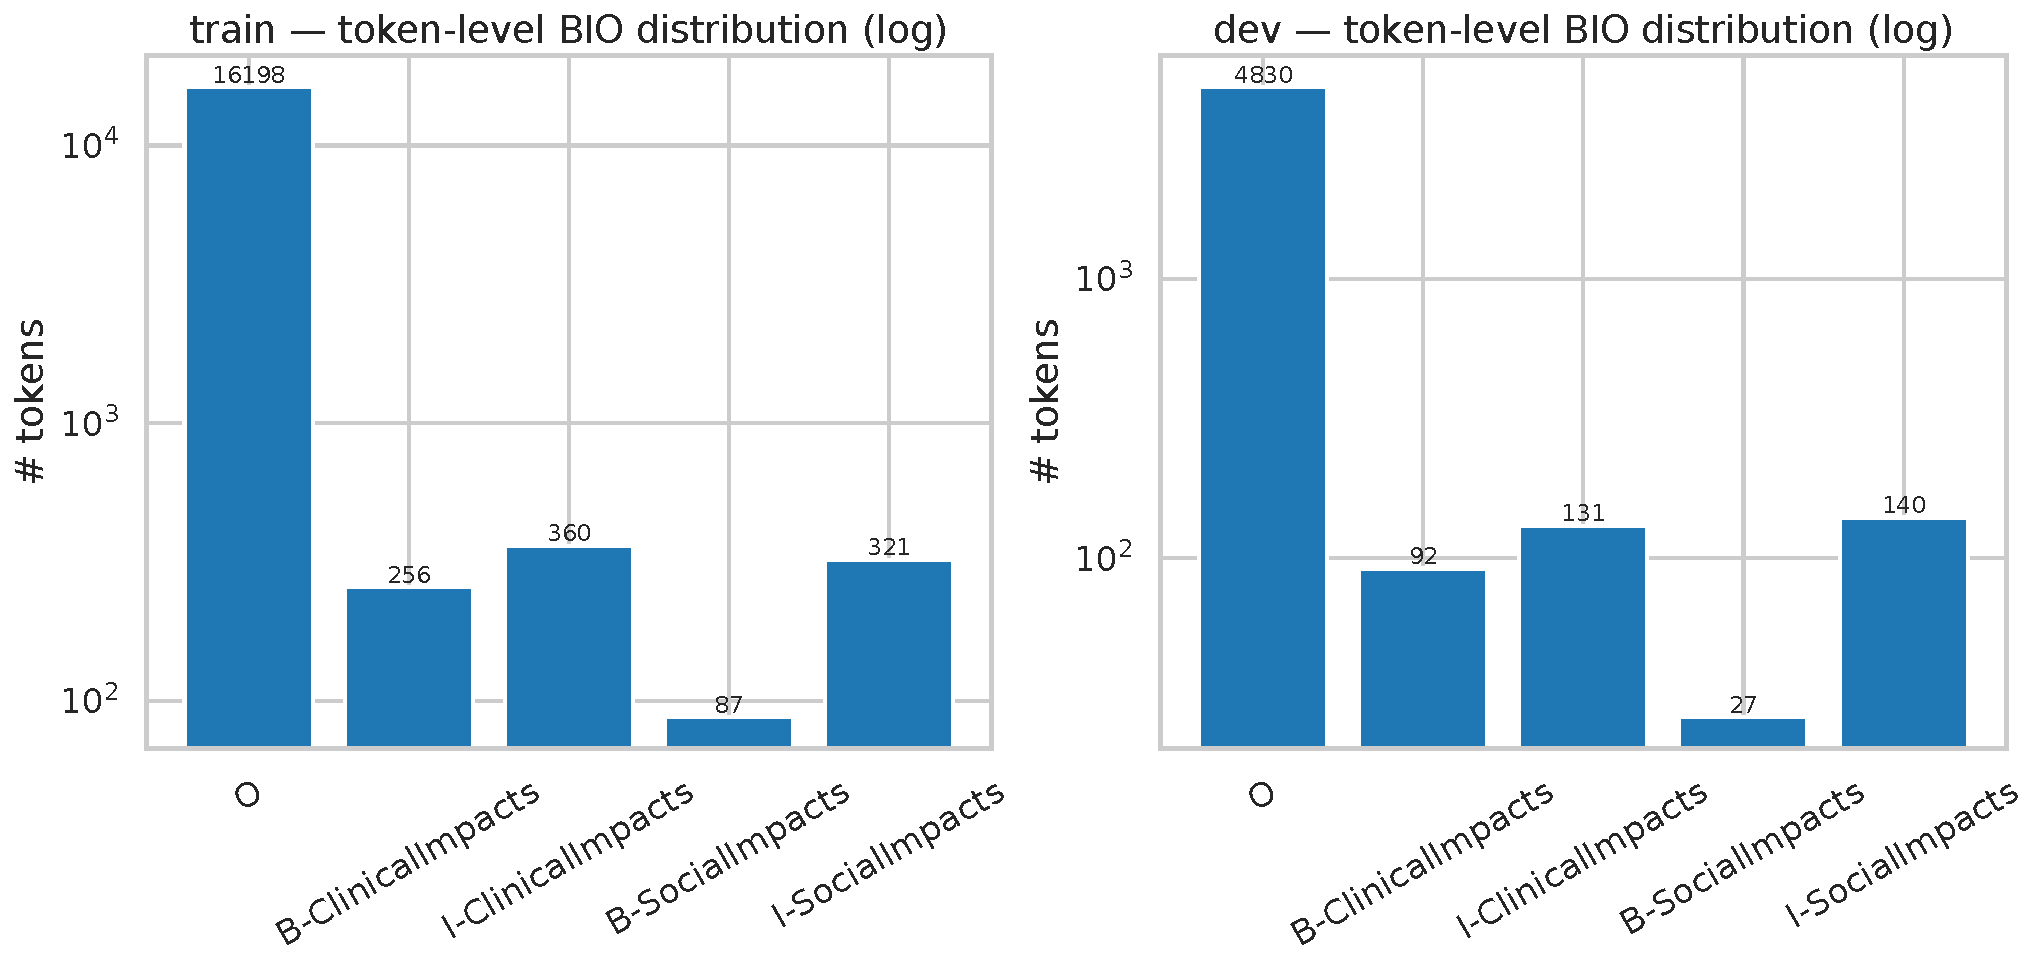
\includegraphics[width=\columnwidth]{01_class_distribution.pdf}
\caption{Token-level BIO distribution on the train and dev splits
(log scale). The \texttt{O} class dominates by a factor of $\sim$$16{:}1$.}
\label{fig:class_dist}
\end{figure}

\begin{figure}[!t]
\centering
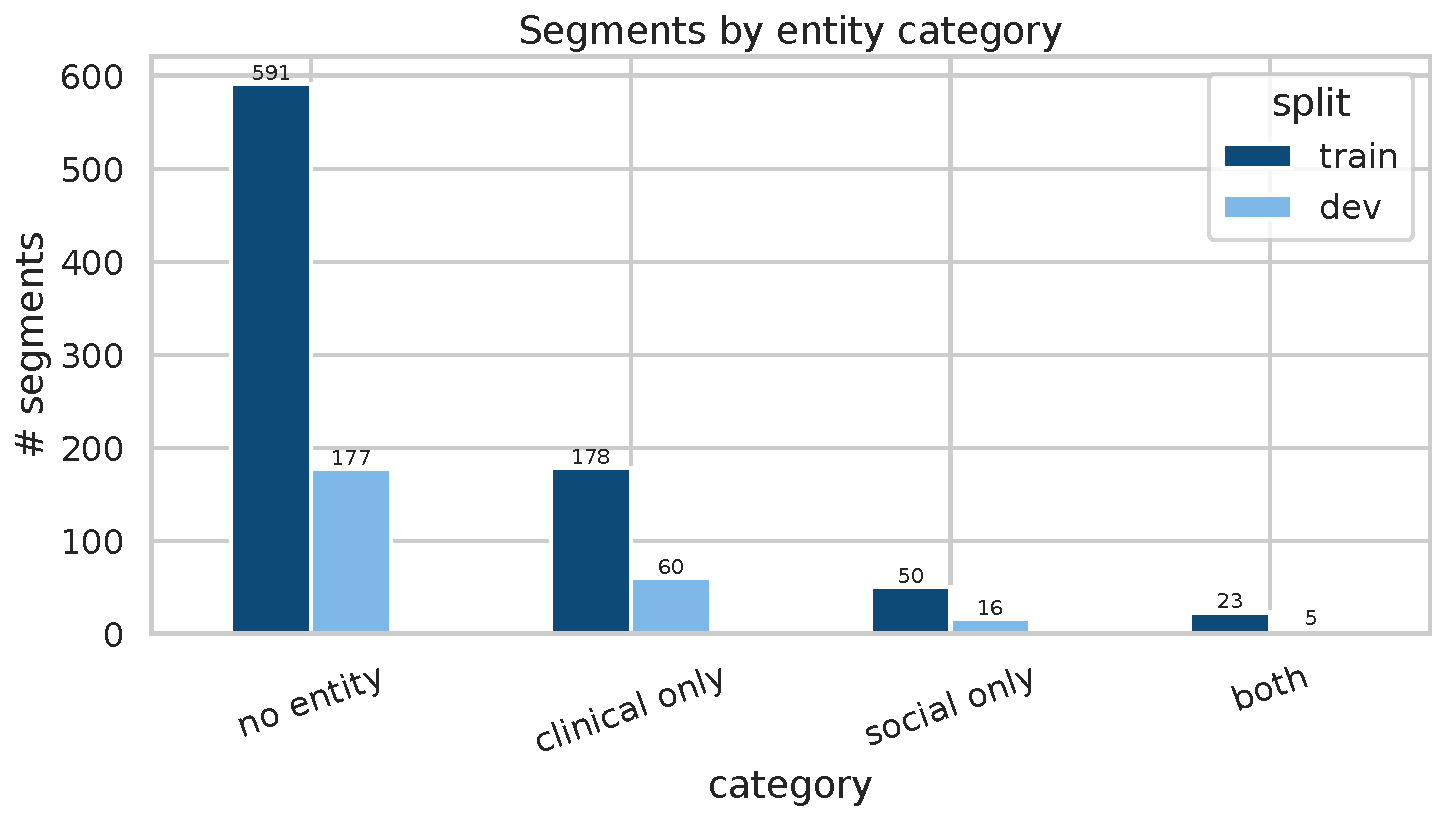
\includegraphics[width=\columnwidth]{04_entity_category.pdf}
\caption{Number of segments per entity category. The \emph{no entity}
class accounts for $70\%$ of train and $68\%$ of dev segments.}
\label{fig:entity_cat}
\end{figure}

\begin{figure}[!t]
\centering
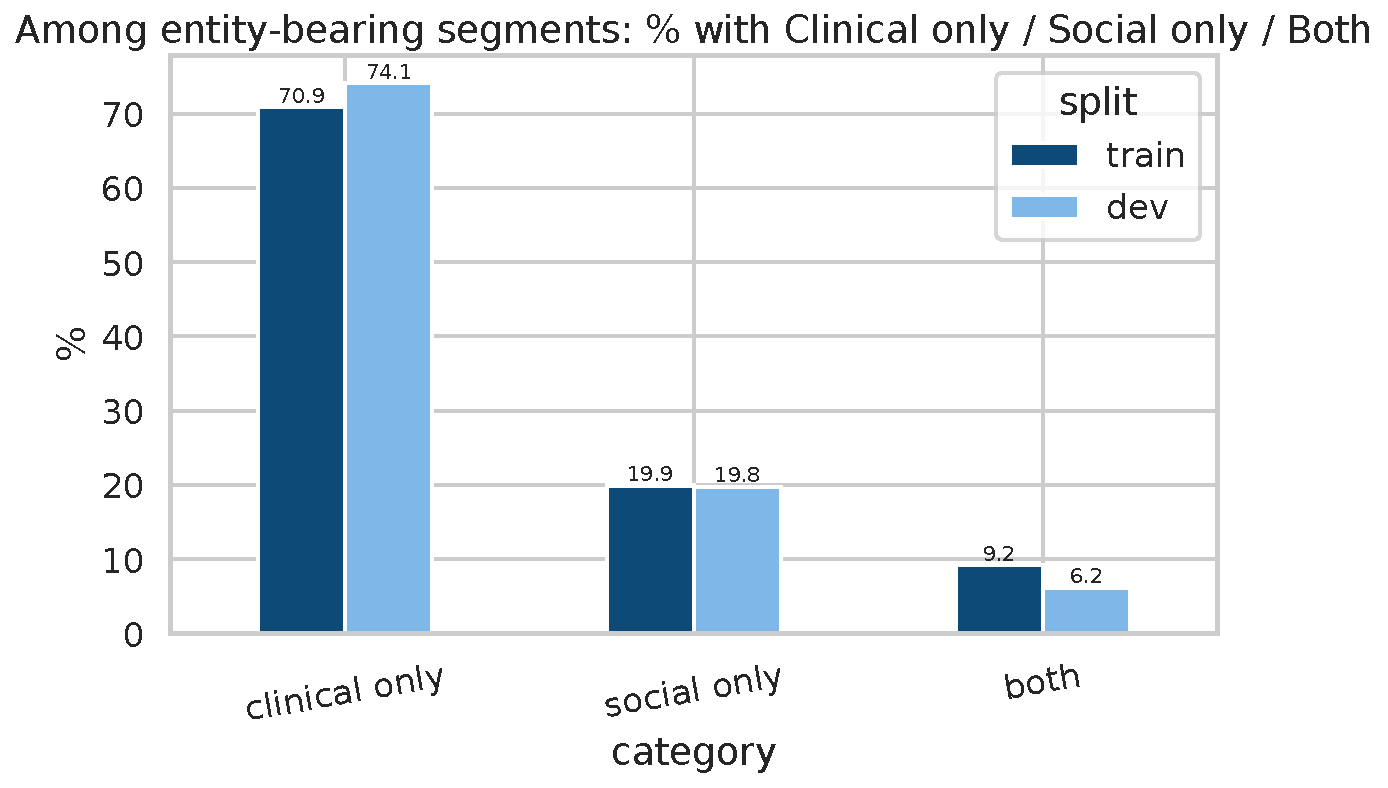
\includegraphics[width=\columnwidth]{06_co_occurrence.pdf}
\caption{Among entity-bearing segments, the share of segments
containing only Clinical, only Social, or both impact types.}
\label{fig:cooccur}
\end{figure}

\subsubsection{Span and segment length}
Most spans are short. The histogram in Fig.~\ref{fig:span_len} shows
that the bulk of both \texttt{ClinicalImpacts} ($n{=}256$ train,
$92$ dev) and \texttt{SocialImpacts} ($n{=}87$ train, $27$ dev)
spans is between one and four tokens long, with a tail extending to
$\sim$$25$ tokens. Train and dev segments fit comfortably within
$256$ tokens (max $123$ and $119$ respectively,
Fig.~\ref{fig:seq_len}), but the test split contains $221$ segments
longer than $300$ tokens, including one outlier of $9{,}009$ tokens.
We therefore set the per-segment maximum length to $256$ during
training, and apply a sliding-window inference scheme on test
segments that exceed this budget.

\begin{figure}[!t]
\centering
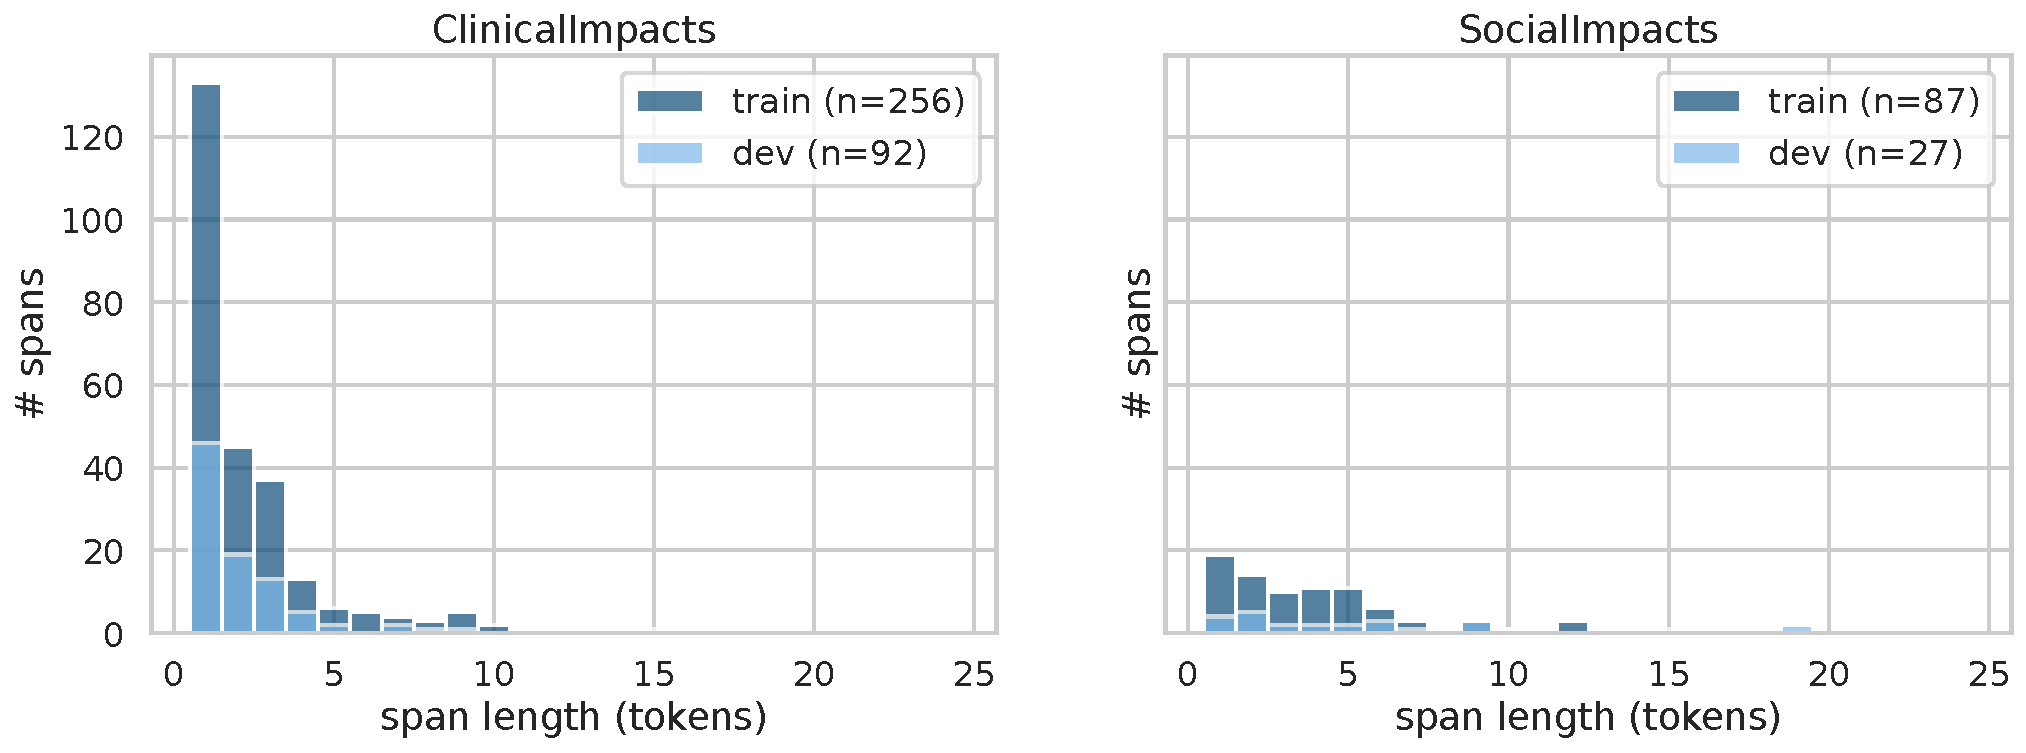
\includegraphics[width=\columnwidth]{03_span_length.pdf}
\caption{Span-length distribution per entity class. Both classes are
heavily concentrated in the $1$--$4$ token range.}
\label{fig:span_len}
\end{figure}

\begin{figure}[!t]
\centering
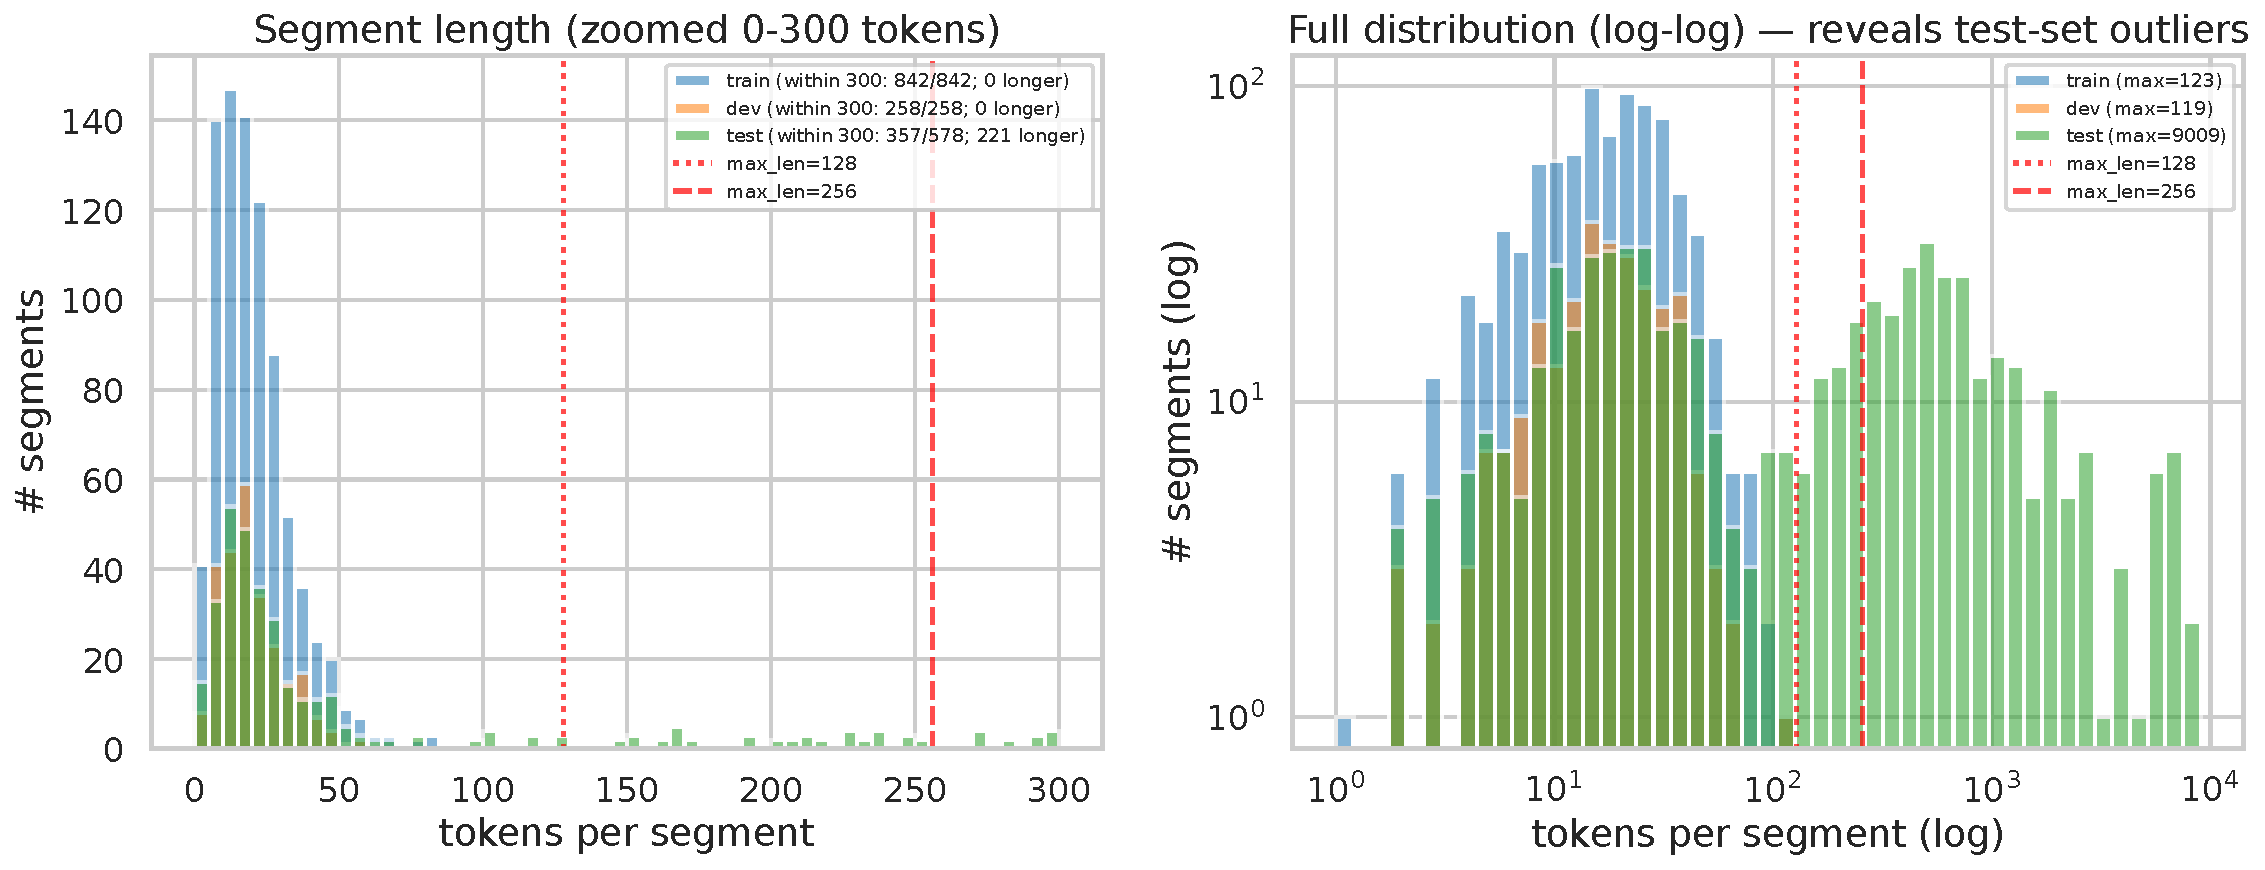
\includegraphics[width=\columnwidth]{02_sequence_length.pdf}
\caption{Segment length in tokens (top: zoomed; bottom: log--log).
Train and dev are bounded by $\sim$$120$ tokens, while $221$ test
segments exceed $300$ tokens, with one outlier at $9{,}009$.}
\label{fig:seq_len}
\end{figure}

\subsubsection{Perspective drift between splits}
The SMM4H-HeaRD task targets first-person, self-reported impacts;
third-person mentions (e.g.~``my friend overdosed'') must remain
untagged. We classified each segment by its dominant grammatical
perspective using a small instruction-tuned LLM and observed a
substantial mismatch between the splits (Fig.~\ref{fig:perspective}):
train and dev each contain $\sim$$45\%$ first-person segments, while
the test split is $71.1\%$ first-person. The annotation rate is also
strongly skewed by perspective: $57.7\%$ of first-person segments
contain an entity, against only $13.0\%$ of third-person and
$6.0\%$ of other (Fig.~\ref{fig:entity_by_persp}). This means a
system trained on the official train/dev splits sees a much larger
fraction of un-annotated, off-task content than it will encounter at
test time; conversely, the test split is more concentrated on the
genuinely targeted perspective. We exploit neither perspective
filtering nor weighting in our experiments and leave this as future
work.

\begin{figure}[!t]
\centering
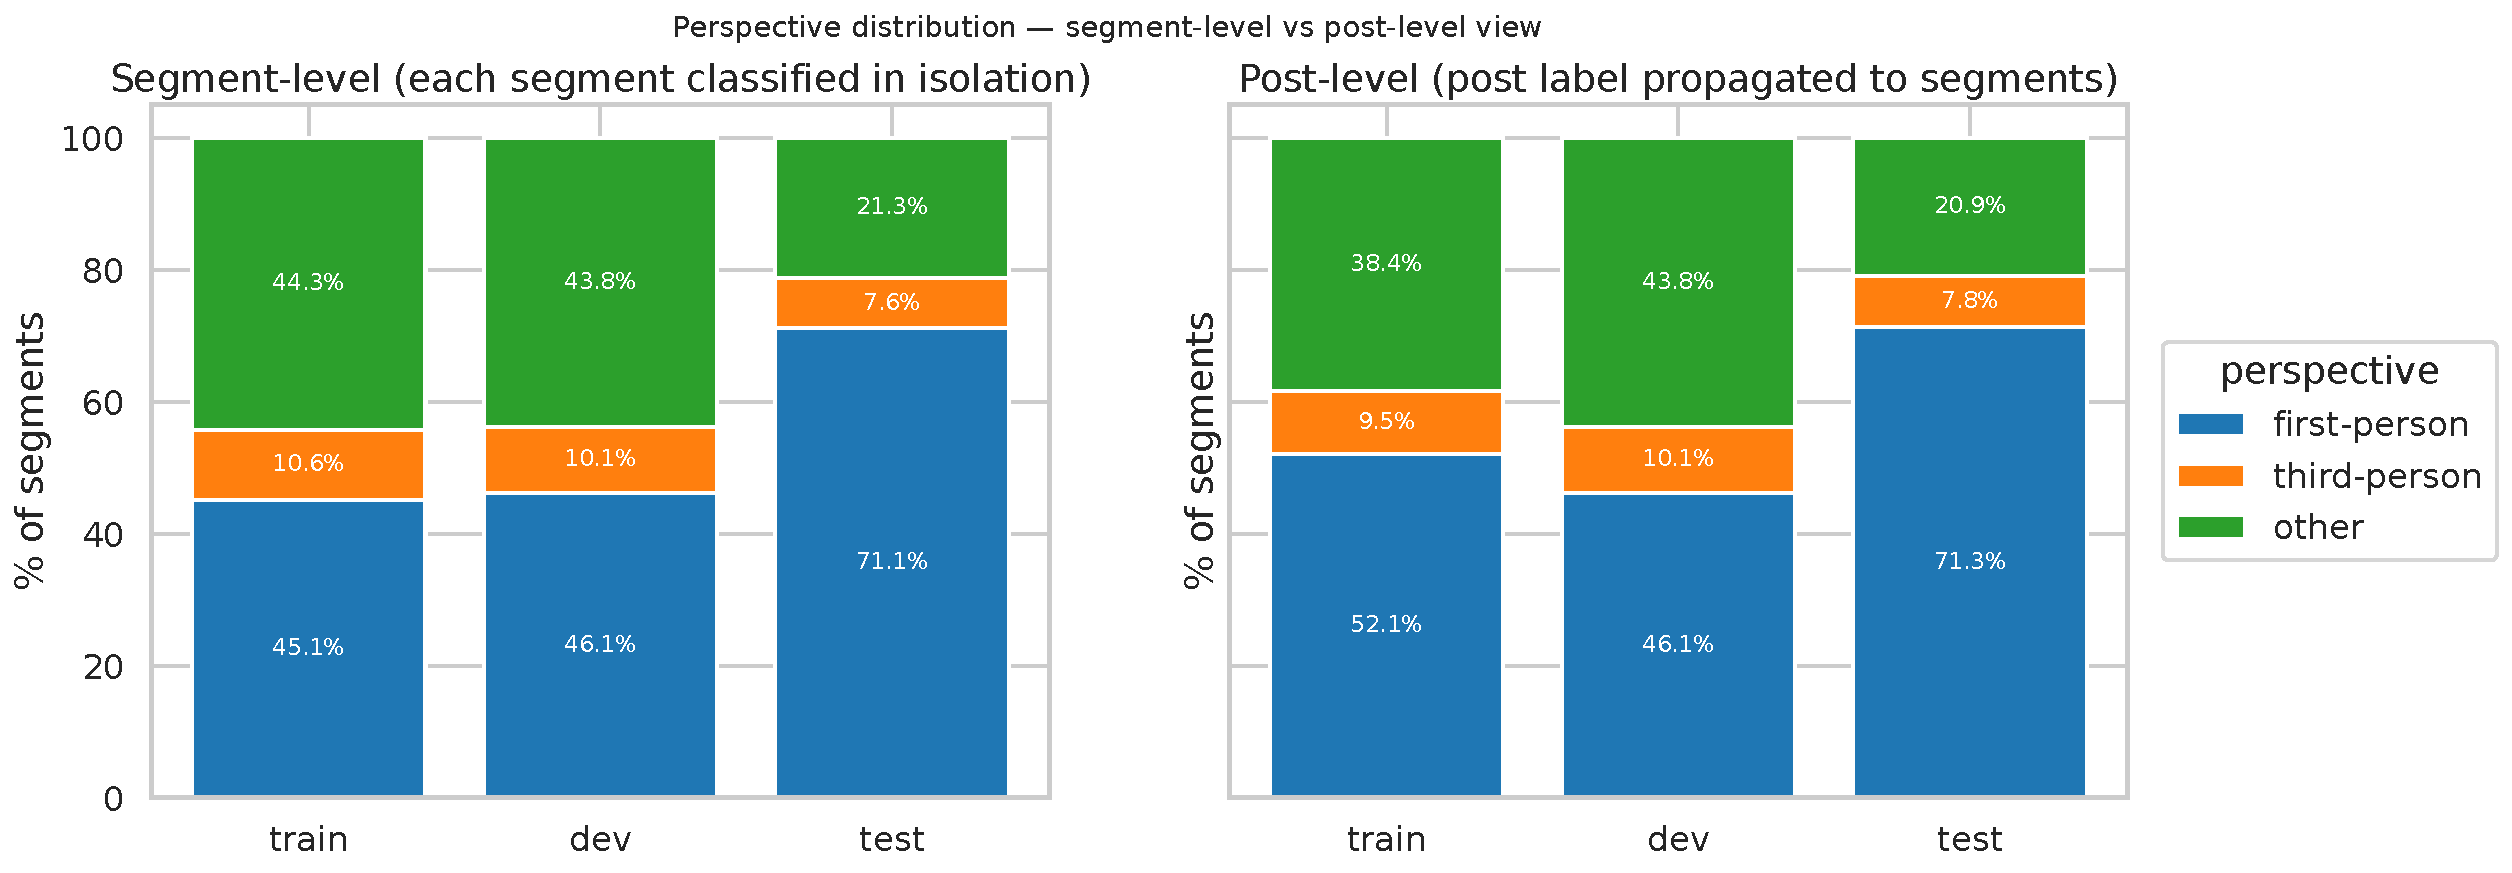
\includegraphics[width=\columnwidth]{10_perspective_segment_vs_post.pdf}
\caption{Post-perspective distribution per split, evaluated both at
the segment and at the post level. The test split is markedly more
first-person than train or dev.}
\label{fig:perspective}
\end{figure}

\begin{figure}[!t]
\centering
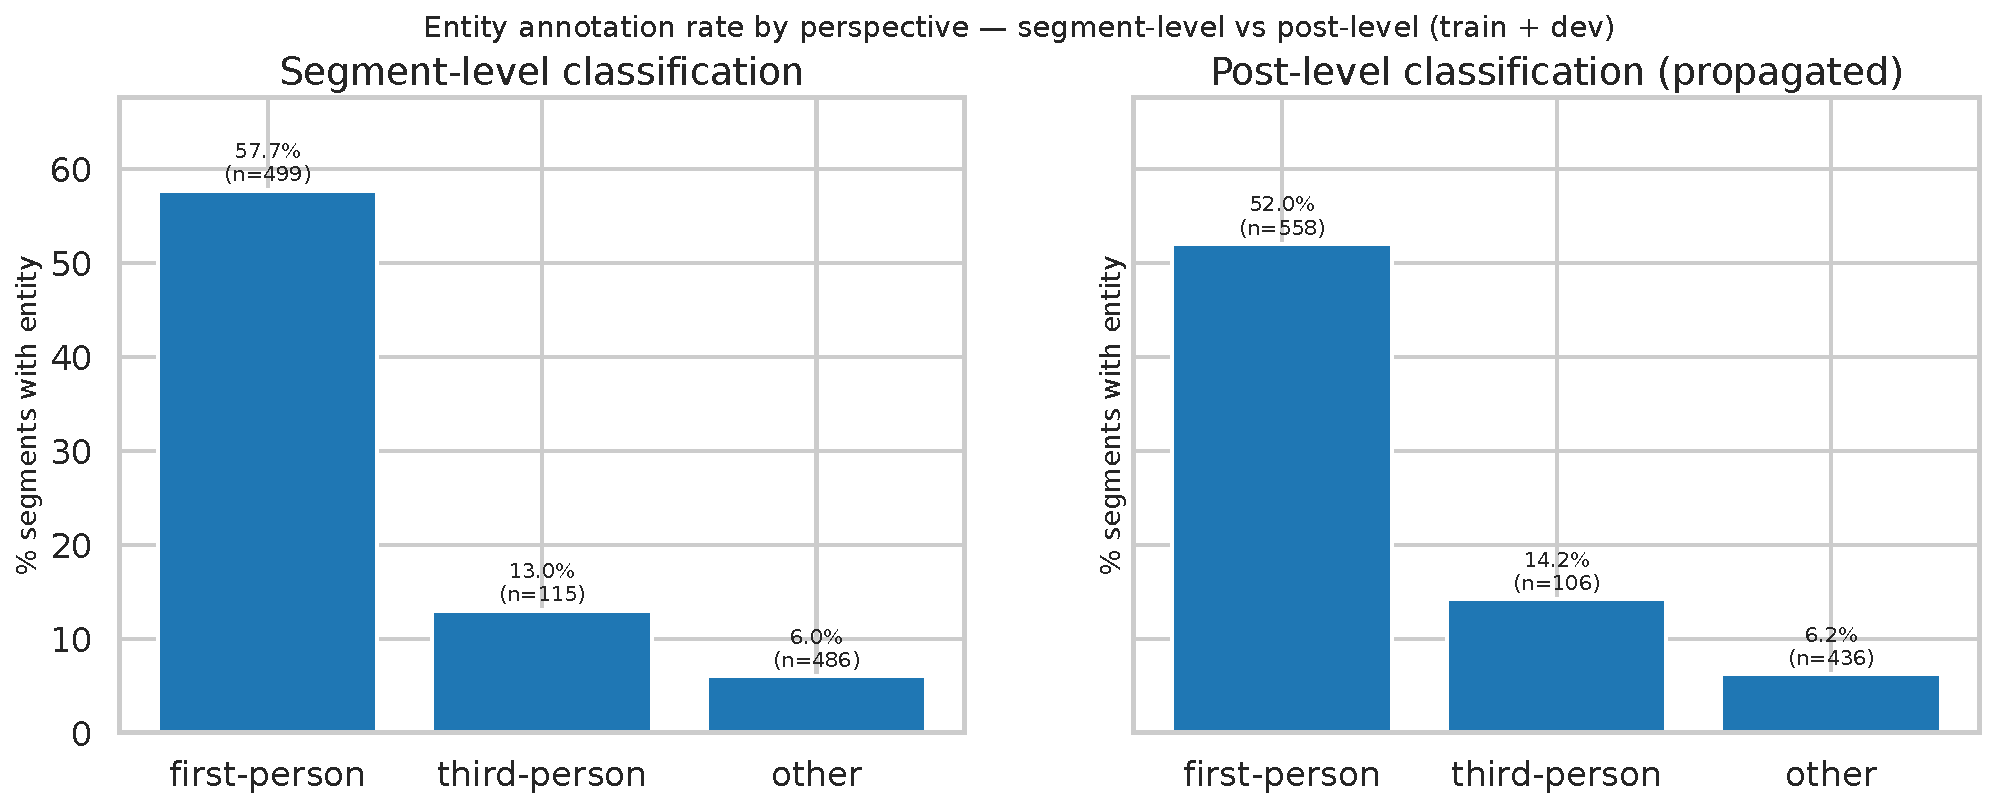
\includegraphics[width=\columnwidth]{11_entity_rate_segment_vs_post.pdf}
\caption{Entity annotation rate by post perspective. First-person
segments are $\sim$$4{\times}$ more likely to contain an annotated
impact span than third-person ones.}
\label{fig:entity_by_persp}
\end{figure}

\subsubsection{Subreddit composition and lexical signature}
As expected, opioid-recovery communities dominate the top of the
subreddit ranking (Fig.~\ref{fig:subreddits}): \texttt{suboxone},
\texttt{opiates}, \texttt{OpiatesRecovery}, and
\texttt{quittingkratom} together account for the bulk of
entity-bearing segments. General-interest subreddits such as
\texttt{AskReddit}, \texttt{pics}, or \texttt{politics} are present in
the corpus but contribute almost no annotated entities, which
reinforces the perspective-mismatch observation above. Word clouds of
the annotated spans (Fig.~\ref{fig:wordclouds}) confirm the lexical
distinction between the two entity types: \texttt{ClinicalImpacts} is
dominated by tokens such as \emph{withdrawal}, \emph{rehab}, and
\emph{addiction}, while \texttt{SocialImpacts} is dominated by
\emph{lost}, \emph{homeless}, \emph{job}, and \emph{family}.

\begin{figure}[!t]
\centering
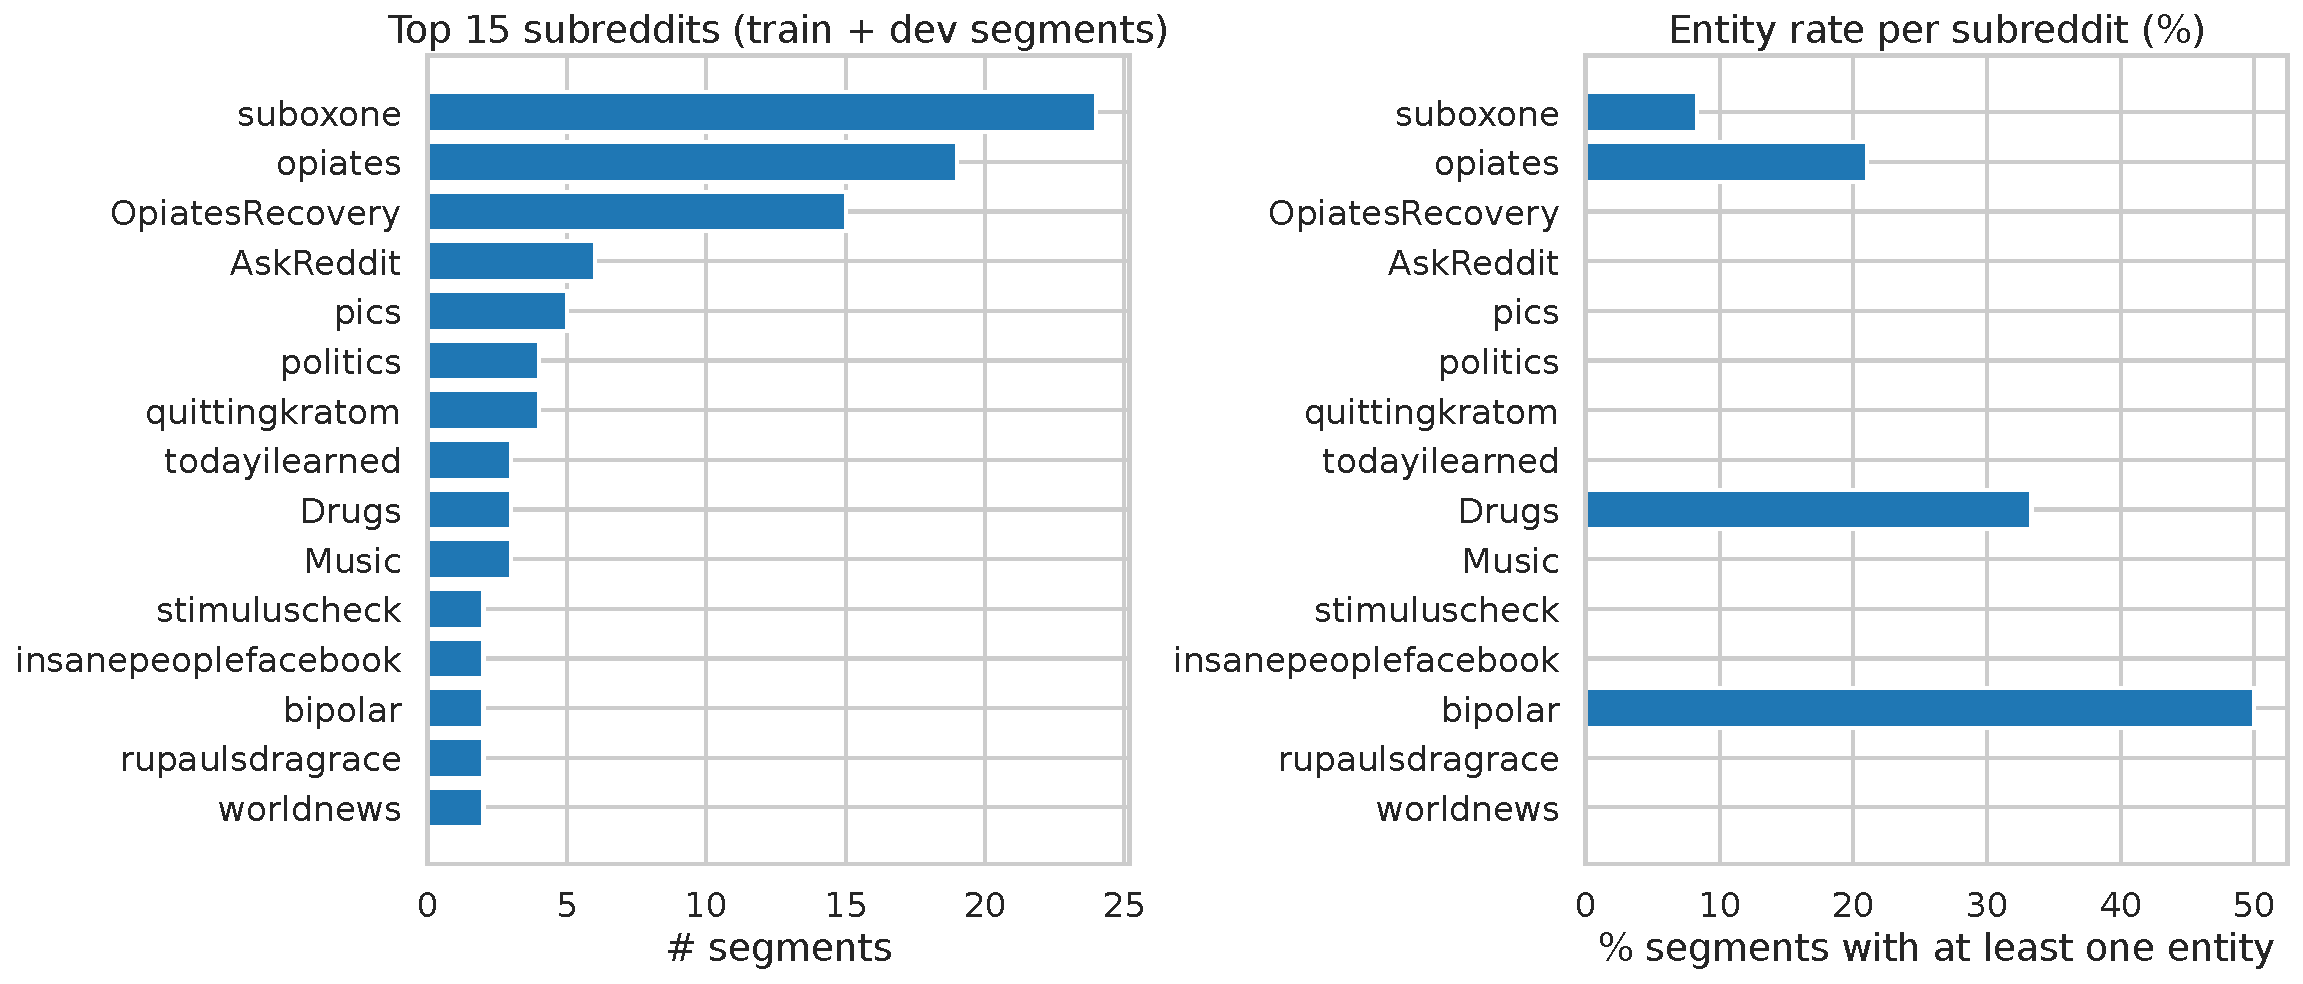
\includegraphics[width=\columnwidth]{05_subreddits.pdf}
\caption{Top-15 subreddits by number of train+dev segments (left) and
their entity-bearing rate (right).}
\label{fig:subreddits}
\end{figure}

\begin{figure}[!t]
\centering
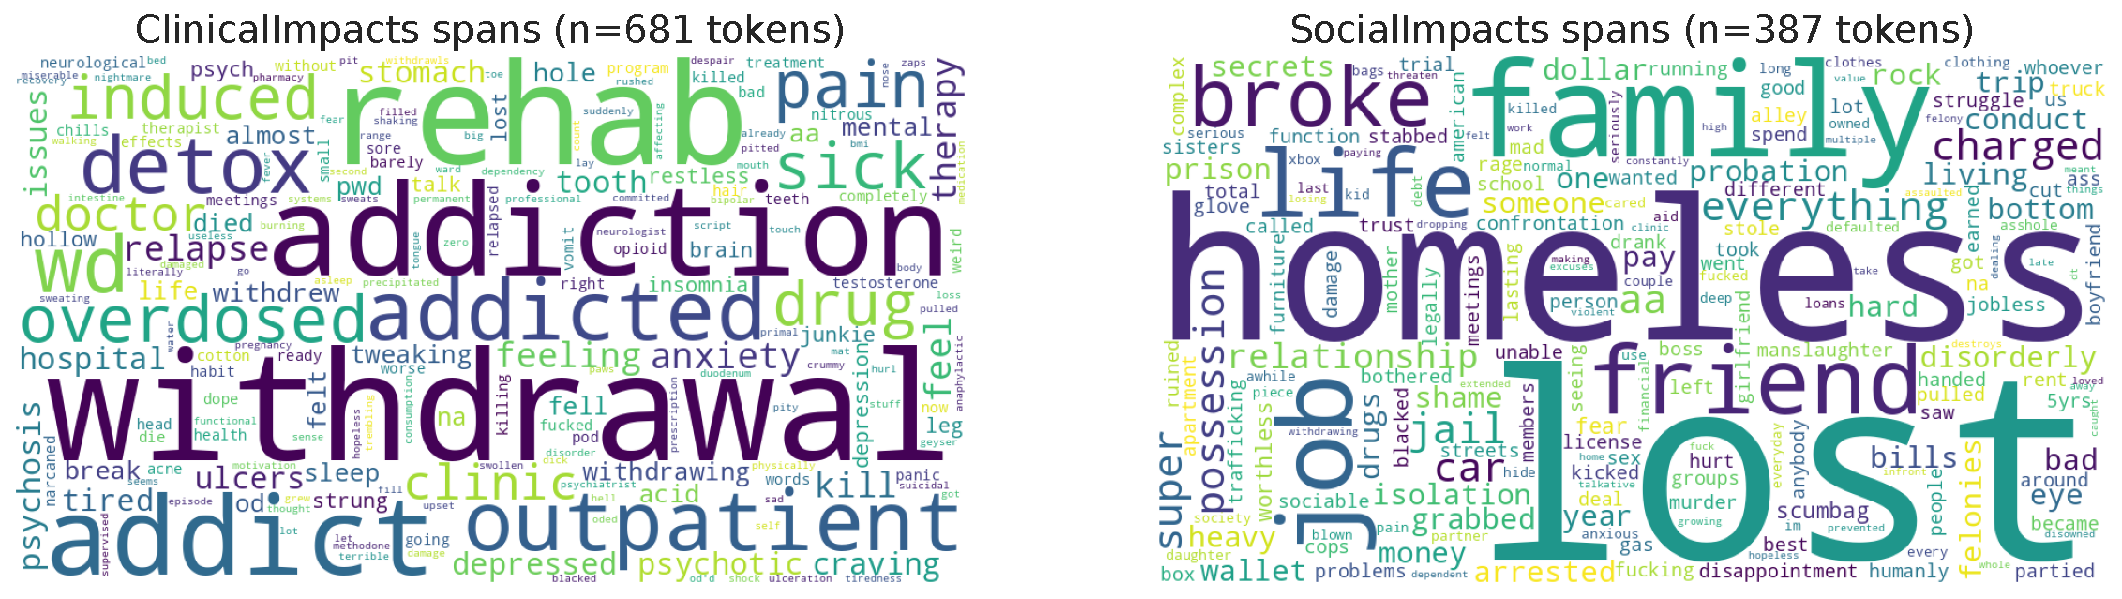
\includegraphics[width=\columnwidth]{07_wordclouds.pdf}
\caption{Word clouds over annotated tokens, separated by entity
class.}
\label{fig:wordclouds}
\end{figure}

\subsection{System design}
\label{ssec:system}
We instantiate four pipelines, all built on top of a shared
encoder-fine-tuning core. The pipelines differ only in how span
boundaries and span types are recovered.

\subsubsection{Direct pipeline}
A single transformer encoder is fine-tuned on the full 5-class BIO
label set and produces token-level predictions in one pass. An
optional CRF head replaces the per-token softmax with a globally
normalised score over full label sequences, decoded by Viterbi at
inference. This is the simplest design and serves as the
encoder-only reference for the other pipelines.

\subsubsection{Two-stage pipeline}
Span detection and span typing are decoupled. A 3-class encoder is
fine-tuned on a collapsed label set (\texttt{O}, \texttt{B-Impact},
\texttt{I-Impact}) so that all impact tokens share a single class.
At inference, the encoder produces impact spans, and each span is
then classified as \texttt{ClinicalImpacts}, \texttt{SocialImpacts},
or \texttt{Neither} by an external classifier. A \texttt{Neither}
verdict reverts the span to \texttt{O}.

\subsubsection{Audit pipeline}
A 5-class encoder produces a full BIO tagging in the same way as in
the direct pipeline. Every non-\texttt{O} predicted span is then sent
to an external classifier with the encoder's current class as a hint;
the classifier may verify, correct, or reject the prediction.
Unlike the two-stage pipeline, the encoder here is solely responsible
for span boundaries, and the external classifier acts as a
post-hoc auditor of the type assignment.

\subsubsection{External classifier}
The external classifier in the two-stage and audit pipelines is one
of two backends:
\begin{itemize}
\item an instruction-tuned causal LLM
(\texttt{Qwen2.5-7B-Instruct} or \texttt{Gemma-3-12B-it}) loaded in
4-bit NF4 precision and prompted in zero-shot or few-shot
($k{=}4$ gold demonstrations per class) regimes;
\item a Support Vector Machine head with PCA-128 dimensionality
reduction and an RBF kernel, trained on encoder span embeddings
extracted offline from the training set.
\end{itemize}
The two backends share the same call interface, which lets us swap
them without changing any other part of the pipeline.

\subsubsection{Training and inference common to all pipelines}
Every encoder is fine-tuned end-to-end on the training split and
selected on the development split using strict micro-F1. We use
either standard cross-entropy, weighted cross-entropy, focal loss, or
the CRF negative log-likelihood as training objective. Layer-wise
learning-rate decay is applied to all DeBERTa-based runs. At
inference, we apply the same sliding-window scheme as for training to
test segments that exceed the maximum length, and we re-aggregate
overlapping windows by majority vote at the token level.

\section{Experiments and Own Contribution}
\label{sec:experiments}
This section walks through every experiment in our ablation in the
order in which one design choice motivated the next. Quantitative dev
and test scores are deferred to Table~\ref{tab:ablation} of
Section~\ref{sec:results}; here we focus on the rationale for each
choice and on the most informative deltas. Throughout the section,
``baseline'' refers to Experiment~01 (Sec.~\ref{ssec:baseline}).

\subsection{Experimental setup common to all runs}
\label{ssec:setup}
Every encoder is fine-tuned on the official $842$-row training split
and selected on the $258$-row development split using strict micro-F1
over the five BIO labels. We use a maximum sequence length of $256$
tokens, a batch size of $16$, $20$ training epochs with a $10\%$
linear warm-up, gradient clipping at $1.0$, and a base learning rate
of $2{\times}10^{-5}$. Word-level BIO labels are propagated to
sub-word tokens via the standard ``first sub-token gets the B/I tag,
others get \texttt{-100}'' convention, and inference labels are
extracted from the first sub-token of each word. All experiments use
seed \texttt{42} unless noted otherwise. Every metric we report is
computed by \texttt{seqeval} on the same data, which guarantees an
identical evaluation protocol across pipelines.

\subsection{Baseline: encoder-only direct pipeline (Exp 01)}
\label{ssec:baseline}
The baseline is a \texttt{mental/mental-roberta-base}~\cite{ji2022mentalbert}
encoder fine-tuned with cross-entropy loss to predict $5$-class BIO
tags directly. We chose this checkpoint for two reasons: it is a
RoBERTa~\cite{liu2019roberta} variant adapted to mental-health
Reddit text, which matches our domain, and its base size
($\sim$$125$\,M parameters) keeps the per-experiment training cost
low enough to run a wide ablation on a single GPU. The baseline
reaches $35.64\%$ strict / $48.89\%$ relaxed F1 on dev and
$36.75\%$ strict / $48.90\%$ relaxed F1 on the Codabench test split.
Two observations follow. First, the $\sim$$13$-point gap between
strict and relaxed scores indicates that the baseline finds entities
in approximately the right places but struggles to predict their
exact boundaries. Second, despite using a domain-adapted checkpoint,
this baseline is roughly $12$ relaxed-F1 points below the
DeBERTa-large baseline reported by the shared-task
organisers~\cite{dey2025inference}, which motivates exploring
stronger backbones, structured decoders, and external classifiers.

\subsection{Direct-pipeline ablation (Exp 02--04, 06)}
\label{ssec:direct}
The first experimental thread keeps the direct (single-encoder)
pipeline shape and varies the loss function, the backbone, and the
decoding head.

\subsubsection{Loss function (Exp 02)}
The class imbalance documented in Sec.~\ref{ssec:dataset} suggests
that the baseline may waste capacity on the dominant \texttt{O}
class. We re-trained the same backbone with two alternative
objectives: (a) weighted cross-entropy with class weights
$[0.05, 1.0, 1.0, 1.0, 1.0]$ for $\{\texttt{O},
\texttt{B-Cli}, \texttt{I-Cli}, \texttt{B-Soc}, \texttt{I-Soc}\}$, and
(b) focal loss~\cite{lin2017focal} with $\gamma{=}2$. Weighted CE
produces a small dev gain ($+0.4$ strict / $+0.4$ relaxed), but
generalises much better to the test split ($+4.3$ strict / $+6.0$
relaxed over the baseline). Focal loss is essentially neutral on
strict F1 and slightly negative on test strict, which suggests that
explicit class weights are a more robust remedy than down-weighting
``easy'' negatives at this dataset scale.

\subsubsection{Stronger backbone with LLRD (Exp 03)}
We replaced \texttt{mental-roberta-base} with
\texttt{microsoft/deberta-v3-base}~\cite{he2023debertav3}, kept focal
loss, and added Layer-wise Learning-Rate Decay~\cite{howard2018ulmfit}
with a per-layer multiplier of $0.9$ from top to bottom. LLRD is a
known stabiliser for DeBERTa fine-tuning because it slows the drift
of the lower (more general) layers while letting the task-specific
head move quickly. The combined change boosts test scores to
$42.40\%$ strict / $55.80\%$ relaxed, a $+5.7$ strict and $+6.9$
relaxed jump over the baseline; this is the largest single-step
improvement in the entire ablation, and the relaxed score here is the
highest test relaxed F1 we observe across all $16$ configurations.

\subsubsection{CRF decoding (Exp 04 --- main contribution)}
\label{sssec:exp04}
Inspired by Lample~\emph{et~al.}~\cite{lample2016neural}, we add a
linear-chain CRF head on top of the DeBERTa-v3 encoder, replacing the
per-token cross-entropy by the CRF negative log-likelihood. The CRF
rules out illegal BIO transitions (e.g.\ \texttt{I-Cli} after
\texttt{B-Soc}) and decodes via Viterbi at inference. The CRF gives
$+3.0$ strict points on the test split over the LLRD baseline of
Exp~03, lifting the test strict score from $42.40\%$ to $45.38\%$
while keeping the relaxed score nearly unchanged ($55.80 \rightarrow
54.20$). The strict-vs-relaxed pattern is consistent with the role of
the CRF: it cleans up boundaries (which strict F1 rewards) without
finding new entities (which relaxed F1 rewards). Exp~04 is therefore
our strongest \emph{single-system} configuration and the encoder
backbone for every downstream LLM and SVM pipeline.

\subsubsection{Multi-seed ensemble (Exp 06)}
We re-trained the Exp~04 (\texttt{DeBERTa-v3-base+CRF}) configuration
with three random seeds ($42$, $123$, $999$) and combined the three
predictions by majority vote at the token level. The ensemble reaches
$44.11\%$ strict / $55.10\%$ relaxed F1 on test, slightly below the
single-seed Exp~04. Token-level voting helps when seeds make
\emph{uncorrelated} mistakes; here all three seeds converge on the
same boundary errors, so the vote has nothing to average over. We
report the ensemble for completeness but use Exp~04 as our final
encoder-only system.

\subsection{LLM-augmented pipelines (Exp 05, 07--09)}
\label{ssec:llm_augmented}
The next experimental thread attaches an instruction-tuned LLM as an
external span classifier on top of the encoder. We explore two
pipeline shapes (Sec.~\ref{ssec:system}):
\begin{itemize}
\item \emph{Two-stage} (Exp 05a, 07a, 08a, 09a). The encoder is
re-trained with a collapsed $3$-class label set
($\{\texttt{O}, \texttt{B-Imp}, \texttt{I-Imp}\}$) and only detects
span boundaries; the LLM types each detected span as
\texttt{ClinicalImpacts}, \texttt{SocialImpacts}, or
\texttt{Neither}.
\item \emph{Audit} (Exp 05b, 07b, 08b, 09b). The $5$-class
\texttt{DeBERTa-v3+CRF} encoder of Exp~04 produces a full BIO
tagging; the LLM is shown the encoder's prediction as a hint and may
verify, correct, or reject it.
\end{itemize}
For each shape we sweep two LLMs
(\texttt{Qwen/Qwen2.5-7B-Instruct} and
\texttt{google/gemma-3-12b-it}, both loaded in $4$-bit NF4 precision
via \texttt{bitsandbytes}~\cite{dettmers2023qlora}) and two prompting
regimes (zero-shot and $4$-shot, with demonstrations mined from gold
training spans). Decoding is greedy, capped at $6$ new tokens; the
post is truncated to $2{,}000$ characters and the candidate span to
$200$ characters.

The strongest LLM configuration is \emph{audit + Gemma-3-12B +
$4$-shot} (Exp~09b), which reaches $42.55\%$ strict / $56.69\%$
relaxed F1 on dev --- the highest \emph{dev} strict score in our
entire ablation. On the test split, however, Exp~09b drops to
$43.20\%$ strict / $52.30\%$ relaxed and is decisively beaten by the
encoder-only Exp~04 ($45.38\%$ / $54.20\%$). We attribute this
inversion to the train/dev~vs.~test distribution shifts of
Sec.~\ref{ssec:dataset}: the $4$-shot demonstrations mined from
training over-fit to the Clinical-heavy, perspective-mixed dev
distribution, and on the more first-person, Social-heavy test split
they no longer help.

Two further patterns emerge. First, all two-stage variants
underperform their audit counterparts at relaxed F1 because the
$3$-class encoder finds slightly worse spans than the
$5$-class~CRF, and the LLM cannot fully recover from upstream
boundary errors. Second, $4$-shot prompting consistently helps
\texttt{Gemma} but hurts \texttt{Qwen} (e.g.~$-0.3$ test strict on
the audit pipeline, $-0.6$ on dev), suggesting that the larger Gemma
model is better at extracting type signal from demonstrations while
the smaller Qwen treats them more as noise.

\subsection{SVM-augmented variant (Exp 10)}
\label{ssec:svm}
To isolate how much of the LLM's contribution comes from world
knowledge that is not already linearly accessible in the encoder's
representation, we replaced the LLM with a classical Support Vector
Machine~\cite{cortes1995svm}. The classifier head is
\texttt{StandardScaler} $\rightarrow$ \texttt{PCA(128)} $\rightarrow$
\texttt{SVC(RBF, class\_weight=balanced)}, with $C$ and $\gamma$
chosen by $5$-fold grid-searched macro-F1, and the input is the
mean-pooled hidden state of the span tokens taken from the encoder
of Exp~04.

The two-stage SVM (Exp~10a) achieves $43.27\%$ strict / $43.50\%$
relaxed on the test split: comparable strict F1 to the LLM
counterparts but markedly weaker relaxed F1, because the small number
of Social-class training spans ($87$) is not enough to robustly
classify the noisy boundaries of the $3$-class encoder. The audit
SVM (Exp~10b) preserves most of the Exp~04 dev numbers
($40.65\%$ strict / $55.91\%$ relaxed) and a $5$-fold macro-F1 of
$1.0$ on gold training embeddings shows that the two classes are
linearly separable in the CRF encoder's feature space, so the SVM
rarely overrides the encoder. This is a useful contrast to the LLM
audits in Exp~09b: when the encoder is already strong, the LLM audit
adds a measurable, if modest, dev gain ($+1.3$ strict over Exp~04)
while the classical SVM audit adds nothing. Both, however, lose to
the encoder on test.

\section{Results and Discussion}
\label{sec:results}

Table~\ref{tab:ablation} collects every configuration we trained or
prompted, together with strict and relaxed F1 on both the development
split and the official Codabench test split. Within each metric, the
best score across the entire ablation is set in bold.

\subsection{Headline result and overall trends}
The strongest single system on the test split is the encoder-only
\emph{DeBERTa-v3-base + CRF} configuration (Exp~04), which reaches
$45.38\%$ strict / $54.20\%$ relaxed F1 --- a $+8.6$ strict and
$+5.3$ relaxed gain over the \texttt{mental-roberta-base} baseline
(Exp~01). The improvement is the cumulative effect of three
modifications: (i)~switching the backbone to
DeBERTa-v3~\cite{he2023debertav3} ($+5.7$ strict on test from
Exp~02a to Exp~03 once weighted CE is replaced by focal loss with
LLRD), (ii)~adding a CRF head with Viterbi decoding~\cite{lample2016neural,
lafferty2001crf} ($+3.0$ strict on test from Exp~03 to Exp~04), and
(iii)~enforcing valid BIO transitions, which closes most of the
strict--relaxed gap (Sec.~\ref{sssec:strict_vs_relaxed}). None of the
LLM-augmented or SVM-augmented variants improves on Exp~04's test
strict F1, although several stay within $1$ point of it.

\subsection{Per-class breakdown}
Table~\ref{tab:per_class} reports relaxed precision, recall, and F1
broken down by entity type for five representative configurations.
The baseline shows a $14$-point gap between
\texttt{ClinicalImpacts} ($54.5\%$) and \texttt{SocialImpacts}
($40.6\%$), driven entirely by the recall side
(Clinical recall $49.3\%$ vs.\ Social $32.9\%$). This matches the
training-set imbalance documented in Sec.~\ref{ssec:dataset}: there
are $\sim$$3{\times}$ as many Clinical spans as Social spans, and the
weakest models simply miss the Social entities. The gap closes
sharply once the backbone is upgraded: by Exp~03 the two classes
agree to within $0.5$ F1 points, and Exp~04 actually flips the
ranking (Social slightly above Clinical at $57.3\%$ vs.\ $57.0\%$).
The gap re-opens by $1$--$2$ points in the LLM and SVM audit
pipelines (Exp~09b, 10b), which suggests that the secondary
classifier is biased towards Clinical and re-introduces the
asymmetry the CRF had erased.

\begin{table}[!t]
\renewcommand{\arraystretch}{1.1}
\caption{Per-class relaxed precision (P), recall (R), and F1 on the
development split for five representative configurations.}
\label{tab:per_class}
\centering
\footnotesize
\setlength{\tabcolsep}{4pt}
\begin{tabular}{l c c c c c c}
\hline
& \multicolumn{3}{c}{\textbf{ClinicalImpacts}} & \multicolumn{3}{c}{\textbf{SocialImpacts}} \\
\cline{2-4}\cline{5-7}
\textbf{Exp} & P & R & F1 & P & R & F1 \\
\hline
01 (m-roberta, CE)            & 0.608 & 0.493 & 0.545 & 0.529 & 0.329 & 0.406 \\
03 (DeBERTa+LLRD)             & 0.652 & 0.462 & 0.541 & 0.664 & 0.449 & 0.536 \\
04 (DeBERTa+CRF)              & 0.692 & 0.484 & 0.570 & 0.743 & 0.467 & 0.574 \\
09b (Gemma audit, $4$-sh.)    & 0.729 & 0.471 & 0.572 & 0.743 & 0.449 & 0.560 \\
10b (SVM audit)               & 0.671 & 0.484 & 0.563 & 0.740 & 0.443 & 0.554 \\
\hline
\end{tabular}
\end{table}

\subsection{Strict vs.\ relaxed F1}
\label{sssec:strict_vs_relaxed}
The strict score requires both the boundaries and the type to be
correct, while the relaxed score only requires any token-level
overlap. The gap between them therefore measures how often the
system finds an entity \emph{near} but not exactly where the
annotators placed it. The baseline has a $13.3$-point strict-relaxed
gap on dev ($35.6$ vs.\ $48.9$); this widens to $19.4$ points in the
LLRD configuration of Exp~03 ($34.5$ vs.\ $53.9$), because the
stronger encoder finds more entity \emph{regions} but with even
noisier boundaries. The CRF closes the gap back to $15.8$ points on
dev and to a strikingly small $8.8$ points on test ($45.4$ vs.\
$54.2$), confirming that the structured decoder's main contribution
is boundary cleaning rather than entity discovery. None of the LLM
or SVM heads further reduces this gap, which is consistent with
their span-level (rather than token-level) operating regime: by
construction they cannot edit boundaries, only re-classify the
spans the encoder has already proposed.

\subsection{Precision/recall asymmetry}
A pattern shared by every system in the table is that recall, not
precision, is the bottleneck. Across Exp~01--Exp~10b on dev,
relaxed precision climbs from $0.58$ to $0.73$ as we improve the
pipeline, but relaxed recall stays in the narrow $0.42$--$0.48$
band. In other words, our systems are progressively more
\emph{conservative}: they hallucinate fewer false-positive impact
spans, but the absolute number of gold spans they discover does not
materially change. We attribute this to the sheer scarcity of
training data --- $343$ Clinical and $87$ Social spans in $842$
posts is too little for the model to learn the long tail of
expressions for ``lost my job'', ``slept on the streets'', etc., so
the unseen variants at test time remain invisible.

\subsection{Comparison to the organisers' baseline and shortcomings}
The strongest baseline reported by the shared-task
organisers~\cite{dey2025inference} is a DeBERTa-large model that
reaches $\sim$$0.61$ relaxed F1 on the same test split. Our best
system (Exp~04) is $\sim$$7$ relaxed-F1 points behind and Exp~09b
is $\sim$$8$ points behind. Three factors plausibly account for the
gap. First, every encoder we used is the \emph{base} variant; given
the consistent $+5$--$+7$ point gain from \texttt{mental-roberta}
to \texttt{deberta-v3-base}, a further jump to
\texttt{deberta-v3-large} is the most likely single source of
remaining improvement. Second, our CRF and LLM audits operate on
\emph{token-level} BIO predictions; the organisers' system uses a
post-hoc span-merging heuristic that recovers contiguous entities
spanning more than a single segment, which our pipeline cannot do
because it processes each released CSV row independently. Third, our
$4$-shot demonstrations are sampled by class only; recent work on
in-context learning suggests that perspective-balanced or
length-balanced sampling would better match the test distribution.
Addressing these points is the natural next step beyond the present
study.

\begin{table*}[!t]
\renewcommand{\arraystretch}{1.15}
\caption{Ablation across all $16$ configurations. Pipeline shapes:
\texttt{D}~=~direct, \texttt{2S}~=~two-stage, \texttt{Au}~=~audit,
\texttt{Ens}~=~ensemble, \texttt{2S/Au+SVM}~=~SVM-augmented
two-stage/audit. CRF and LLRD columns are \texttt{Y/N}. ``External''
gives the span classifier used in two-stage, audit, and SVM
pipelines. Best per metric in bold.}
\label{tab:ablation}
\centering
\footnotesize
\begin{tabular}{l l l l c c l c c c c}
\hline
\textbf{Exp} & \textbf{Pipe} & \textbf{Backbone} & \textbf{Loss}
& \textbf{CRF} & \textbf{LLRD} & \textbf{External}
& \textbf{Dev S} & \textbf{Dev R} & \textbf{Test S} & \textbf{Test R} \\
\hline
01  & D    & mental-roberta-base       & CE          & N & N & ---                          & 0.3564 & 0.4889 & 0.3675 & 0.4890 \\
02a & D    & mental-roberta-base       & W-CE        & N & N & ---                          & 0.3603 & 0.4928 & 0.4096 & 0.5490 \\
02b & D    & mental-roberta-base       & Focal       & N & N & ---                          & 0.3387 & 0.4924 & 0.3362 & 0.5070 \\
03  & D    & deberta-v3-base           & Focal       & N & Y & ---                          & 0.3446 & 0.5386 & 0.4240 & \textbf{0.5580} \\
04  & D    & deberta-v3-base           & CRF NLL     & Y & Y & ---                          & 0.4130 & \textbf{0.5714} & \textbf{0.4538} & 0.5420 \\
06  & Ens  & deberta-v3-base $\times 3$ & CRF NLL    & Y & Y & ---                          & 0.4098 & 0.5649 & 0.4411 & 0.5510 \\
\hline
05a & 2S   & deberta-v3-base (3-cls)   & Focal       & N & Y & Qwen2.5-7B, zero-shot        & 0.3941 & 0.4230 & 0.4206 & 0.4490 \\
05b & Au   & deberta-v3-base           & CRF NLL     & Y & Y & Qwen2.5-7B, zero-shot        & 0.3860 & 0.5407 & 0.4426 & 0.5490 \\
07a & 2S   & deberta-v3-base (3-cls)   & Focal       & N & Y & Qwen2.5-7B, $4$-shot         & 0.3814 & 0.4309 & 0.4340 & 0.4830 \\
07b & Au   & deberta-v3-base           & CRF NLL     & Y & Y & Qwen2.5-7B, $4$-shot         & 0.3797 & 0.5369 & 0.4400 & 0.5520 \\
08a & 2S   & deberta-v3-base (3-cls)   & Focal       & N & Y & Gemma-3-12B, zero-shot       & 0.3824 & 0.4207 & 0.3946 & 0.4180 \\
08b & Au   & deberta-v3-base           & CRF NLL     & Y & Y & Gemma-3-12B, zero-shot       & 0.3877 & 0.5502 & 0.4000 & 0.4960 \\
09a & 2S   & deberta-v3-base (3-cls)   & Focal       & N & Y & Gemma-3-12B, $4$-shot        & 0.4076 & 0.4376 & 0.4279 & 0.4440 \\
09b & Au   & deberta-v3-base           & CRF NLL     & Y & Y & Gemma-3-12B, $4$-shot        & \textbf{0.4255} & 0.5669 & 0.4320 & 0.5230 \\
\hline
10a & 2S+SVM & deberta-v3-base (3-cls) & Focal       & N & Y & SVM (RBF, PCA-128)          & 0.3571 & 0.3674 & 0.4327 & 0.4350 \\
10b & Au+SVM & deberta-v3-base         & CRF NLL     & Y & Y & SVM (RBF, PCA-128)          & 0.4065 & 0.5591 & ---    & ---    \\
\hline
\end{tabular}
\end{table*}


% An example of a floating figure using the graphicx package.
% Note that \label must occur AFTER (or within) \caption.
% For figures, \caption should occur after the \includegraphics.
% Note that IEEEtran v1.7 and later has special internal code that
% is designed to preserve the operation of \label within \caption
% even when the captionsoff option is in effect. However, because
% of issues like this, it may be the safest practice to put all your
% \label just after \caption rather than within \caption{}.
%
% Reminder: the "draftcls" or "draftclsnofoot", not "draft", class
% option should be used if it is desired that the figures are to be
% displayed while in draft mode.
%
%\begin{figure}[!t]
%\centering
%\includegraphics[width=2.5in]{myfigure}
% where an .eps filename suffix will be assumed under latex, 
% and a .pdf suffix will be assumed for pdflatex; or what has been declared
% via \DeclareGraphicsExtensions.
%\caption{Simulation results for the network.}
%\label{fig_sim}
%\end{figure}

% Note that the IEEE typically puts floats only at the top, even when this
% results in a large percentage of a column being occupied by floats.


% An example of a double column floating figure using two subfigures.
% (The subfig.sty package must be loaded for this to work.)
% The subfigure \label commands are set within each subfloat command,
% and the \label for the overall figure must come after \caption.
% \hfil is used as a separator to get equal spacing.
% Watch out that the combined width of all the subfigures on a 
% line do not exceed the text width or a line break will occur.
%
%\begin{figure*}[!t]
%\centering
%\subfloat[Case I]{\includegraphics[width=2.5in]{box}%
%\label{fig_first_case}}
%\hfil
%\subfloat[Case II]{\includegraphics[width=2.5in]{box}%
%\label{fig_second_case}}
%\caption{Simulation results for the network.}
%\label{fig_sim}
%\end{figure*}
%
% Note that often IEEE papers with subfigures do not employ subfigure
% captions (using the optional argument to \subfloat[]), but instead will
% reference/describe all of them (a), (b), etc., within the main caption.
% Be aware that for subfig.sty to generate the (a), (b), etc., subfigure
% labels, the optional argument to \subfloat must be present. If a
% subcaption is not desired, just leave its contents blank,
% e.g., \subfloat[].


% An example of a floating table. Note that, for IEEE style tables, the
% \caption command should come BEFORE the table and, given that table
% captions serve much like titles, are usually capitalized except for words
% such as a, an, and, as, at, but, by, for, in, nor, of, on, or, the, to
% and up, which are usually not capitalized unless they are the first or
% last word of the caption. Table text will default to \footnotesize as
% the IEEE normally uses this smaller font for tables.
% The \label must come after \caption as always.
%
%\begin{table}[!t]
%% increase table row spacing, adjust to taste
%\renewcommand{\arraystretch}{1.3}
% if using array.sty, it might be a good idea to tweak the value of
% \extrarowheight as needed to properly center the text within the cells
%\caption{An Example of a Table}
%\label{table_example}
%\centering
%% Some packages, such as MDW tools, offer better commands for making tables
%% than the plain LaTeX2e tabular which is used here.
%\begin{tabular}{|c||c|}
%\hline
%One & Two\\
%\hline
%Three & Four\\
%\hline
%\end{tabular}
%\end{table}


% Note that the IEEE does not put floats in the very first column
% - or typically anywhere on the first page for that matter. Also,
% in-text middle ("here") positioning is typically not used, but it
% is allowed and encouraged for Computer Society conferences (but
% not Computer Society journals). Most IEEE journals/conferences use
% top floats exclusively. 
% Note that, LaTeX2e, unlike IEEE journals/conferences, places
% footnotes above bottom floats. This can be corrected via the
% \fnbelowfloat command of the stfloats package.




\section{Conclusion and Future Work}
\label{sec:conclusion}

We presented a comparative study of four NER pipeline shapes on the
SMM4H-HeaRD~2026 Task~7 dataset: a direct encoder, a two-stage
detect-then-classify pipeline, an audit pipeline that lets a
secondary classifier verify the encoder's output, and a lightweight
SVM variant of the same audit shape. Across $16$ configurations, the
strongest single system on the official Codabench test split is
\emph{DeBERTa-v3-base + linear-chain CRF} (Exp~04), which reaches
$45.38\%$ strict and $54.20\%$ relaxed F1, $+8.6$ and $+5.3$ points
above the \texttt{mental-roberta-base} baseline. Returning to the
research questions of Sec.~\ref{sec:introduction}, we find that:
(\textbf{RQ1}) decoupling span detection from span typing does not
improve test F1 over a well-decoded $5$-class CRF; the best LLM- and
SVM-augmented pipelines stay within $1$ test strict point of Exp~04
without surpassing it. (\textbf{RQ2}) On the development split a
$4$-shot Gemma-3-12B audit gains $+1.3$ strict F1 over the encoder,
but this advantage does not transfer to the test split, suggesting
that span-level external classifiers are at best a marginal addition
to a strong CRF backbone on this dataset. The dominant remaining
error is low recall on rare social-impact expressions, driven by the
small training set ($87$ Social spans) and the perspective-shift
between train/dev and test.

The most promising directions for future work follow directly from
the gap to the organisers'
DeBERTa-large baseline~\cite{dey2025inference}. First, scaling the
encoder to \texttt{deberta-v3-large} and adding domain-adaptive
pre-training on Reddit substance-use posts would address the
recall-bound regime we observed. Second, reintroducing a span-merging
post-processing step that aggregates predictions across the
sentence-level test rows would remove an artificial limitation of
our segment-by-segment inference. Third, replacing the class-only
$4$-shot demonstration sampler with a perspective and length-aware
retriever would mitigate the dev/test prompt mismatch we identified.





% if have a single appendix:
%\appendix[Proof of the Zonklar Equations]
% or
%\appendix  % for no appendix heading
% do not use \section anymore after \appendix, only \section*
% is possibly needed

% use appendices with more than one appendix
% then use \section to start each appendix
% you must declare a \section before using any
% \subsection or using \label (\appendices by itself
% starts a section numbered zero.)
%


% Can use something like this to put references on a page
% by themselves when using endfloat and the captionsoff option.
\ifCLASSOPTIONcaptionsoff
  \newpage
\fi



% trigger a \newpage just before the given reference
% number - used to balance the columns on the last page
% adjust value as needed - may need to be readjusted if
% the document is modified later
%\IEEEtriggeratref{8}
% The "triggered" command can be changed if desired:
%\IEEEtriggercmd{\enlargethispage{-5in}}

% references section

% can use a bibliography generated by BibTeX as a .bbl file
% BibTeX documentation can be easily obtained at:
% http://mirror.ctan.org/biblio/bibtex/contrib/doc/
% The IEEEtran BibTeX style support page is at:
% http://www.michaelshell.org/tex/ieeetran/bibtex/
%\bibliographystyle{IEEEtran}
% argument is your BibTeX string definitions and bibliography database(s)
%\bibliography{IEEEabrv,../bib/paper}
%
% <OR> manually copy in the resultant .bbl file
% set second argument of \begin to the number of references
% (used to reserve space for the reference number labels box)
\begin{thebibliography}{99}

\bibitem{dey2025inference}
S.~K. Dey, J.~M. Powell, A.~Ismail, J.~Perrone, and A.~Sarker,
``Inference gap in domain expertise and machine intelligence in named entity
recognition: Creation of and insights from a substance use-related dataset,''
in \emph{Biocomputing 2026: Proceedings of the Pacific Symposium}.\hskip 1em plus
  0.5em minus 0.4em\relax World Scientific, 2025, pp.~12--26.

\bibitem{devlin2019bert}
J.~Devlin, M.-W. Chang, K.~Lee, and K.~Toutanova,
``BERT: Pre-training of deep bidirectional transformers for language
understanding,'' in \emph{Proc. NAACL-HLT}, 2019, pp.~4171--4186.

\bibitem{liu2019roberta}
Y.~Liu, M.~Ott, N.~Goyal, J.~Du, M.~Joshi, D.~Chen, O.~Levy, M.~Lewis,
L.~Zettlemoyer, and V.~Stoyanov,
``RoBERTa: A robustly optimized BERT pretraining approach,''
\emph{arXiv preprint arXiv:1907.11692}, 2019.

\bibitem{he2023debertav3}
P.~He, J.~Gao, and W.~Chen,
``DeBERTaV3: Improving DeBERTa using ELECTRA-style pre-training with
gradient-disentangled embedding sharing,''
in \emph{Proc. Int. Conf. Learning Representations (ICLR)}, 2023.

\bibitem{ji2022mentalbert}
S.~Ji, T.~Zhang, L.~Ansari, J.~Fu, P.~Tiwari, and E.~Cambria,
``MentalBERT: Publicly available pretrained language models for mental
healthcare,'' in \emph{Proc. 13th Language Resources and Evaluation Conf.
(LREC)}, 2022, pp.~7184--7190.

\bibitem{lafferty2001crf}
J.~Lafferty, A.~McCallum, and F.~C.~N. Pereira,
``Conditional random fields: Probabilistic models for segmenting and labeling
sequence data,''
in \emph{Proc. 18th Int. Conf. Machine Learning (ICML)}, 2001, pp.~282--289.

\bibitem{lample2016neural}
G.~Lample, M.~Ballesteros, S.~Subramanian, K.~Kawakami, and C.~Dyer,
``Neural architectures for named entity recognition,''
in \emph{Proc. NAACL-HLT}, 2016, pp.~260--270.

\bibitem{tjong2003conll}
E.~F. Tjong Kim Sang and F.~De~Meulder,
``Introduction to the CoNLL-2003 shared task: Language-independent named
entity recognition,''
in \emph{Proc. 7th Conf. Natural Language Learning (CoNLL)}, 2003,
pp.~142--147.

\bibitem{lin2017focal}
T.-Y. Lin, P.~Goyal, R.~Girshick, K.~He, and P.~Doll\'ar,
``Focal loss for dense object detection,''
in \emph{Proc. IEEE Int. Conf. Computer Vision (ICCV)}, 2017,
pp.~2980--2988.

\bibitem{howard2018ulmfit}
J.~Howard and S.~Ruder,
``Universal language model fine-tuning for text classification,''
in \emph{Proc. 56th Annu. Meeting of the Association for Computational
Linguistics (ACL)}, 2018, pp.~328--339.

\bibitem{brown2020fewshot}
T.~B. Brown \emph{et al.},
``Language models are few-shot learners,''
in \emph{Advances in Neural Information Processing Systems (NeurIPS)},
vol.~33, 2020, pp.~1877--1901.

\bibitem{dettmers2023qlora}
T.~Dettmers, A.~Pagnoni, A.~Holtzman, and L.~Zettlemoyer,
``QLoRA: Efficient finetuning of quantized LLMs,''
in \emph{Advances in Neural Information Processing Systems (NeurIPS)},
vol.~36, 2023.

\bibitem{cortes1995svm}
C.~Cortes and V.~Vapnik,
``Support-vector networks,''
\emph{Machine Learning}, vol.~20, no.~3, pp.~273--297, 1995.

\end{thebibliography}

% biography section
% 
% If you have an EPS/PDF photo (graphicx package needed) extra braces are
% needed around the contents of the optional argument to biography to prevent
% the LaTeX parser from getting confused when it sees the complicated
% \includegraphics command within an optional argument. (You could create
% your own custom macro containing the \includegraphics command to make things
% simpler here.)
%\begin{IEEEbiography}[{\includegraphics[width=1in,height=1.25in,clip,keepaspectratio]{mshell}}]{Michael Shell}
% or if you just want to reserve a space for a photo:


% You can push biographies down or up by placing
% a \vfill before or after them. The appropriate
% use of \vfill depends on what kind of text is
% on the last page and whether or not the columns
% are being equalized.

%\vfill

% Can be used to pull up biographies so that the bottom of the last one
% is flush with the other column.
%\enlargethispage{-5in}



% that's all folks
\end{document}


